% Options for packages loaded elsewhere
\PassOptionsToPackage{unicode}{hyperref}
\PassOptionsToPackage{hyphens}{url}
%
\documentclass[
]{article}
\usepackage{amsmath,amssymb}
\usepackage{iftex}
\ifPDFTeX
  \usepackage[T1]{fontenc}
  \usepackage[utf8]{inputenc}
  \usepackage{textcomp} % provide euro and other symbols
\else % if luatex or xetex
  \usepackage{unicode-math} % this also loads fontspec
  \defaultfontfeatures{Scale=MatchLowercase}
  \defaultfontfeatures[\rmfamily]{Ligatures=TeX,Scale=1}
\fi
\usepackage{lmodern}
\ifPDFTeX\else
  % xetex/luatex font selection
\fi
% Use upquote if available, for straight quotes in verbatim environments
\IfFileExists{upquote.sty}{\usepackage{upquote}}{}
\IfFileExists{microtype.sty}{% use microtype if available
  \usepackage[]{microtype}
  \UseMicrotypeSet[protrusion]{basicmath} % disable protrusion for tt fonts
}{}
\makeatletter
\@ifundefined{KOMAClassName}{% if non-KOMA class
  \IfFileExists{parskip.sty}{%
    \usepackage{parskip}
  }{% else
    \setlength{\parindent}{0pt}
    \setlength{\parskip}{6pt plus 2pt minus 1pt}}
}{% if KOMA class
  \KOMAoptions{parskip=half}}
\makeatother
\usepackage{xcolor}
\usepackage[margin=1in]{geometry}
\usepackage{color}
\usepackage{fancyvrb}
\newcommand{\VerbBar}{|}
\newcommand{\VERB}{\Verb[commandchars=\\\{\}]}
\DefineVerbatimEnvironment{Highlighting}{Verbatim}{commandchars=\\\{\}}
% Add ',fontsize=\small' for more characters per line
\usepackage{framed}
\definecolor{shadecolor}{RGB}{248,248,248}
\newenvironment{Shaded}{\begin{snugshade}}{\end{snugshade}}
\newcommand{\AlertTok}[1]{\textcolor[rgb]{0.94,0.16,0.16}{#1}}
\newcommand{\AnnotationTok}[1]{\textcolor[rgb]{0.56,0.35,0.01}{\textbf{\textit{#1}}}}
\newcommand{\AttributeTok}[1]{\textcolor[rgb]{0.13,0.29,0.53}{#1}}
\newcommand{\BaseNTok}[1]{\textcolor[rgb]{0.00,0.00,0.81}{#1}}
\newcommand{\BuiltInTok}[1]{#1}
\newcommand{\CharTok}[1]{\textcolor[rgb]{0.31,0.60,0.02}{#1}}
\newcommand{\CommentTok}[1]{\textcolor[rgb]{0.56,0.35,0.01}{\textit{#1}}}
\newcommand{\CommentVarTok}[1]{\textcolor[rgb]{0.56,0.35,0.01}{\textbf{\textit{#1}}}}
\newcommand{\ConstantTok}[1]{\textcolor[rgb]{0.56,0.35,0.01}{#1}}
\newcommand{\ControlFlowTok}[1]{\textcolor[rgb]{0.13,0.29,0.53}{\textbf{#1}}}
\newcommand{\DataTypeTok}[1]{\textcolor[rgb]{0.13,0.29,0.53}{#1}}
\newcommand{\DecValTok}[1]{\textcolor[rgb]{0.00,0.00,0.81}{#1}}
\newcommand{\DocumentationTok}[1]{\textcolor[rgb]{0.56,0.35,0.01}{\textbf{\textit{#1}}}}
\newcommand{\ErrorTok}[1]{\textcolor[rgb]{0.64,0.00,0.00}{\textbf{#1}}}
\newcommand{\ExtensionTok}[1]{#1}
\newcommand{\FloatTok}[1]{\textcolor[rgb]{0.00,0.00,0.81}{#1}}
\newcommand{\FunctionTok}[1]{\textcolor[rgb]{0.13,0.29,0.53}{\textbf{#1}}}
\newcommand{\ImportTok}[1]{#1}
\newcommand{\InformationTok}[1]{\textcolor[rgb]{0.56,0.35,0.01}{\textbf{\textit{#1}}}}
\newcommand{\KeywordTok}[1]{\textcolor[rgb]{0.13,0.29,0.53}{\textbf{#1}}}
\newcommand{\NormalTok}[1]{#1}
\newcommand{\OperatorTok}[1]{\textcolor[rgb]{0.81,0.36,0.00}{\textbf{#1}}}
\newcommand{\OtherTok}[1]{\textcolor[rgb]{0.56,0.35,0.01}{#1}}
\newcommand{\PreprocessorTok}[1]{\textcolor[rgb]{0.56,0.35,0.01}{\textit{#1}}}
\newcommand{\RegionMarkerTok}[1]{#1}
\newcommand{\SpecialCharTok}[1]{\textcolor[rgb]{0.81,0.36,0.00}{\textbf{#1}}}
\newcommand{\SpecialStringTok}[1]{\textcolor[rgb]{0.31,0.60,0.02}{#1}}
\newcommand{\StringTok}[1]{\textcolor[rgb]{0.31,0.60,0.02}{#1}}
\newcommand{\VariableTok}[1]{\textcolor[rgb]{0.00,0.00,0.00}{#1}}
\newcommand{\VerbatimStringTok}[1]{\textcolor[rgb]{0.31,0.60,0.02}{#1}}
\newcommand{\WarningTok}[1]{\textcolor[rgb]{0.56,0.35,0.01}{\textbf{\textit{#1}}}}
\usepackage{graphicx}
\makeatletter
\def\maxwidth{\ifdim\Gin@nat@width>\linewidth\linewidth\else\Gin@nat@width\fi}
\def\maxheight{\ifdim\Gin@nat@height>\textheight\textheight\else\Gin@nat@height\fi}
\makeatother
% Scale images if necessary, so that they will not overflow the page
% margins by default, and it is still possible to overwrite the defaults
% using explicit options in \includegraphics[width, height, ...]{}
\setkeys{Gin}{width=\maxwidth,height=\maxheight,keepaspectratio}
% Set default figure placement to htbp
\makeatletter
\def\fps@figure{htbp}
\makeatother
\setlength{\emergencystretch}{3em} % prevent overfull lines
\providecommand{\tightlist}{%
  \setlength{\itemsep}{0pt}\setlength{\parskip}{0pt}}
\setcounter{secnumdepth}{-\maxdimen} % remove section numbering
\ifLuaTeX
  \usepackage{selnolig}  % disable illegal ligatures
\fi
\IfFileExists{bookmark.sty}{\usepackage{bookmark}}{\usepackage{hyperref}}
\IfFileExists{xurl.sty}{\usepackage{xurl}}{} % add URL line breaks if available
\urlstyle{same}
\hypersetup{
  pdftitle={HUDM6052 Psychometric II Homework\_04},
  pdfauthor={Chenguang Pan},
  hidelinks,
  pdfcreator={LaTeX via pandoc}}

\title{HUDM6052 Psychometric II Homework\_04}
\author{Chenguang Pan}
\date{2023-11-14}

\begin{document}
\maketitle

\setcounter{tocdepth}{4}
\tableofcontents

\hypertarget{q1-a-parameters-estimation}{%
\subsection{Q1-a-Parameters-Estimation}\label{q1-a-parameters-estimation}}

\emph{Fit the 1PL, 2PL, and 3PL models\ldots report the estimated item
parameters in separated tables}

\textbf{My Solution:}\\
To make the layout concise and good-looking, I intentionally omitted the
codes for data cleaning and some instant display of running outcomes. I
attached the estimated item parameters from all three models into one
table to save space.

\begin{Shaded}
\begin{Highlighting}[]
\SpecialCharTok{\textgreater{}} \CommentTok{\# load the binary response dataset}
\ErrorTok{\textgreater{}} \FunctionTok{library}\NormalTok{(mirt)}
\SpecialCharTok{\textgreater{}}\NormalTok{ df }\OtherTok{\textless{}{-}} \FunctionTok{read.csv}\NormalTok{(}\StringTok{"/Users/panpeter/Desktop/PhD\_Learning/HUDM6052 Psychometric II/HUDM6052\_Psychometic\_II/assignment 4/binary\_reponses.csv"}\NormalTok{)}
\SpecialCharTok{\textgreater{}}\NormalTok{ df }\OtherTok{\textless{}{-}}\NormalTok{ df[,}\SpecialCharTok{{-}}\DecValTok{1}\NormalTok{]}
\SpecialCharTok{\textgreater{}} 
\ErrorTok{\textgreater{}} \CommentTok{\# {-}{-}{-}{-}{-}{-}{-}{-}{-}{-}{-}{-}{-}{-}{-}{-}{-}{-}{-}{-}{-}{-}{-}{-}{-}{-}{-}{-}{-}{-}{-}{-}{-}{-}{-}{-}{-}{-}{-}{-}{-}{-}{-}{-}{-}{-}{-}{-}{-}{-}}
\ErrorTok{\textgreater{}} \CommentTok{\#                       Run 1PL}
\ErrorTok{\textgreater{}} \CommentTok{\# {-}{-}{-}{-}{-}{-}{-}{-}{-}{-}{-}{-}{-}{-}{-}{-}{-}{-}{-}{-}{-}{-}{-}{-}{-}{-}{-}{-}{-}{-}{-}{-}{-}{-}{-}{-}{-}{-}{-}{-}{-}{-}{-}{-}{-}{-}{-}{-}{-}{-}}
\ErrorTok{\textgreater{}} 
\ErrorTok{\textgreater{}} \CommentTok{\# specify the model for 33 items loading on 1 dimension}
\ErrorTok{\textgreater{}} \CommentTok{\# and constrain all the item slope to be equal for 1PL estimation}
\ErrorTok{\textgreater{}}\NormalTok{ spec }\OtherTok{\textless{}{-}} \StringTok{\textquotesingle{}F = 1{-}33}
\StringTok{+ CONSTRAIN = (1{-}33, a1)\textquotesingle{}}
\SpecialCharTok{\textgreater{}} 
\ErrorTok{\textgreater{}} \CommentTok{\# estimated the model}
\ErrorTok{\textgreater{}} \CommentTok{\# since I constrained all slopes to be equal, here the argument "2PL" is safe}
\ErrorTok{\textgreater{}}\NormalTok{ irt\_1pl }\OtherTok{\textless{}{-}} \FunctionTok{mirt}\NormalTok{(df, }\AttributeTok{model =}\NormalTok{ spec, }\AttributeTok{itemtype =} \StringTok{"2PL"}\NormalTok{, }\AttributeTok{SE=}\NormalTok{T)}
\NormalTok{Iteration}\SpecialCharTok{:} \DecValTok{1}\NormalTok{, Log}\SpecialCharTok{{-}}\NormalTok{Lik}\SpecialCharTok{:} \SpecialCharTok{{-}}\FloatTok{20276.377}\NormalTok{, Max}\SpecialCharTok{{-}}\NormalTok{Change}\SpecialCharTok{:} \FloatTok{0.18304}\NormalTok{Iteration}\SpecialCharTok{:} \DecValTok{2}\NormalTok{, Log}\SpecialCharTok{{-}}\NormalTok{Lik}\SpecialCharTok{:} \SpecialCharTok{{-}}\FloatTok{20265.381}\NormalTok{, Max}\SpecialCharTok{{-}}\NormalTok{Change}\SpecialCharTok{:} \FloatTok{0.02242}\NormalTok{Iteration}\SpecialCharTok{:} \DecValTok{3}\NormalTok{, Log}\SpecialCharTok{{-}}\NormalTok{Lik}\SpecialCharTok{:} \SpecialCharTok{{-}}\FloatTok{20262.846}\NormalTok{, Max}\SpecialCharTok{{-}}\NormalTok{Change}\SpecialCharTok{:} \FloatTok{0.01549}\NormalTok{Iteration}\SpecialCharTok{:} \DecValTok{4}\NormalTok{, Log}\SpecialCharTok{{-}}\NormalTok{Lik}\SpecialCharTok{:} \SpecialCharTok{{-}}\FloatTok{20260.664}\NormalTok{, Max}\SpecialCharTok{{-}}\NormalTok{Change}\SpecialCharTok{:} \FloatTok{0.00521}\NormalTok{Iteration}\SpecialCharTok{:} \DecValTok{5}\NormalTok{, Log}\SpecialCharTok{{-}}\NormalTok{Lik}\SpecialCharTok{:} \SpecialCharTok{{-}}\FloatTok{20260.483}\NormalTok{, Max}\SpecialCharTok{{-}}\NormalTok{Change}\SpecialCharTok{:} \FloatTok{0.00380}\NormalTok{Iteration}\SpecialCharTok{:} \DecValTok{6}\NormalTok{, Log}\SpecialCharTok{{-}}\NormalTok{Lik}\SpecialCharTok{:} \SpecialCharTok{{-}}\FloatTok{20260.385}\NormalTok{, Max}\SpecialCharTok{{-}}\NormalTok{Change}\SpecialCharTok{:} \FloatTok{0.00376}\NormalTok{Iteration}\SpecialCharTok{:} \DecValTok{7}\NormalTok{, Log}\SpecialCharTok{{-}}\NormalTok{Lik}\SpecialCharTok{:} \SpecialCharTok{{-}}\FloatTok{20260.298}\NormalTok{, Max}\SpecialCharTok{{-}}\NormalTok{Change}\SpecialCharTok{:} \FloatTok{0.00225}\NormalTok{Iteration}\SpecialCharTok{:} \DecValTok{8}\NormalTok{, Log}\SpecialCharTok{{-}}\NormalTok{Lik}\SpecialCharTok{:} \SpecialCharTok{{-}}\FloatTok{20260.275}\NormalTok{, Max}\SpecialCharTok{{-}}\NormalTok{Change}\SpecialCharTok{:} \FloatTok{0.00153}\NormalTok{Iteration}\SpecialCharTok{:} \DecValTok{9}\NormalTok{, Log}\SpecialCharTok{{-}}\NormalTok{Lik}\SpecialCharTok{:} \SpecialCharTok{{-}}\FloatTok{20260.262}\NormalTok{, Max}\SpecialCharTok{{-}}\NormalTok{Change}\SpecialCharTok{:} \FloatTok{0.00112}\NormalTok{Iteration}\SpecialCharTok{:} \DecValTok{10}\NormalTok{, Log}\SpecialCharTok{{-}}\NormalTok{Lik}\SpecialCharTok{:} \SpecialCharTok{{-}}\FloatTok{20260.230}\NormalTok{, Max}\SpecialCharTok{{-}}\NormalTok{Change}\SpecialCharTok{:} \FloatTok{0.00026}\NormalTok{Iteration}\SpecialCharTok{:} \DecValTok{11}\NormalTok{, Log}\SpecialCharTok{{-}}\NormalTok{Lik}\SpecialCharTok{:} \SpecialCharTok{{-}}\FloatTok{20260.229}\NormalTok{, Max}\SpecialCharTok{{-}}\NormalTok{Change}\SpecialCharTok{:} \FloatTok{0.00070}\NormalTok{Iteration}\SpecialCharTok{:} \DecValTok{12}\NormalTok{, Log}\SpecialCharTok{{-}}\NormalTok{Lik}\SpecialCharTok{:} \SpecialCharTok{{-}}\FloatTok{20260.228}\NormalTok{, Max}\SpecialCharTok{{-}}\NormalTok{Change}\SpecialCharTok{:} \FloatTok{0.00018}\NormalTok{Iteration}\SpecialCharTok{:} \DecValTok{13}\NormalTok{, Log}\SpecialCharTok{{-}}\NormalTok{Lik}\SpecialCharTok{:} \SpecialCharTok{{-}}\FloatTok{20260.228}\NormalTok{, Max}\SpecialCharTok{{-}}\NormalTok{Change}\SpecialCharTok{:} \FloatTok{0.00017}\NormalTok{Iteration}\SpecialCharTok{:} \DecValTok{14}\NormalTok{, Log}\SpecialCharTok{{-}}\NormalTok{Lik}\SpecialCharTok{:} \SpecialCharTok{{-}}\FloatTok{20260.228}\NormalTok{, Max}\SpecialCharTok{{-}}\NormalTok{Change}\SpecialCharTok{:} \FloatTok{0.00064}\NormalTok{Iteration}\SpecialCharTok{:} \DecValTok{15}\NormalTok{, Log}\SpecialCharTok{{-}}\NormalTok{Lik}\SpecialCharTok{:} \SpecialCharTok{{-}}\FloatTok{20260.226}\NormalTok{, Max}\SpecialCharTok{{-}}\NormalTok{Change}\SpecialCharTok{:} \FloatTok{0.00014}\NormalTok{Iteration}\SpecialCharTok{:} \DecValTok{16}\NormalTok{, Log}\SpecialCharTok{{-}}\NormalTok{Lik}\SpecialCharTok{:} \SpecialCharTok{{-}}\FloatTok{20260.226}\NormalTok{, Max}\SpecialCharTok{{-}}\NormalTok{Change}\SpecialCharTok{:} \FloatTok{0.00012}\NormalTok{Iteration}\SpecialCharTok{:} \DecValTok{17}\NormalTok{, Log}\SpecialCharTok{{-}}\NormalTok{Lik}\SpecialCharTok{:} \SpecialCharTok{{-}}\FloatTok{20260.226}\NormalTok{, Max}\SpecialCharTok{{-}}\NormalTok{Change}\SpecialCharTok{:} \FloatTok{0.00047}\NormalTok{Iteration}\SpecialCharTok{:} \DecValTok{18}\NormalTok{, Log}\SpecialCharTok{{-}}\NormalTok{Lik}\SpecialCharTok{:} \SpecialCharTok{{-}}\FloatTok{20260.224}\NormalTok{, Max}\SpecialCharTok{{-}}\NormalTok{Change}\SpecialCharTok{:} \FloatTok{0.00043}\NormalTok{Iteration}\SpecialCharTok{:} \DecValTok{19}\NormalTok{, Log}\SpecialCharTok{{-}}\NormalTok{Lik}\SpecialCharTok{:} \SpecialCharTok{{-}}\FloatTok{20260.224}\NormalTok{, Max}\SpecialCharTok{{-}}\NormalTok{Change}\SpecialCharTok{:} \FloatTok{0.00042}\NormalTok{Iteration}\SpecialCharTok{:} \DecValTok{20}\NormalTok{, Log}\SpecialCharTok{{-}}\NormalTok{Lik}\SpecialCharTok{:} \SpecialCharTok{{-}}\FloatTok{20260.223}\NormalTok{, Max}\SpecialCharTok{{-}}\NormalTok{Change}\SpecialCharTok{:} \FloatTok{0.00011}\NormalTok{Iteration}\SpecialCharTok{:} \DecValTok{21}\NormalTok{, Log}\SpecialCharTok{{-}}\NormalTok{Lik}\SpecialCharTok{:} \SpecialCharTok{{-}}\FloatTok{20260.223}\NormalTok{, Max}\SpecialCharTok{{-}}\NormalTok{Change}\SpecialCharTok{:} \FloatTok{0.00030}\NormalTok{Iteration}\SpecialCharTok{:} \DecValTok{22}\NormalTok{, Log}\SpecialCharTok{{-}}\NormalTok{Lik}\SpecialCharTok{:} \SpecialCharTok{{-}}\FloatTok{20260.222}\NormalTok{, Max}\SpecialCharTok{{-}}\NormalTok{Change}\SpecialCharTok{:} \FloatTok{0.00015}\NormalTok{Iteration}\SpecialCharTok{:} \DecValTok{23}\NormalTok{, Log}\SpecialCharTok{{-}}\NormalTok{Lik}\SpecialCharTok{:} \SpecialCharTok{{-}}\FloatTok{20260.222}\NormalTok{, Max}\SpecialCharTok{{-}}\NormalTok{Change}\SpecialCharTok{:} \FloatTok{0.00040}\NormalTok{Iteration}\SpecialCharTok{:} \DecValTok{24}\NormalTok{, Log}\SpecialCharTok{{-}}\NormalTok{Lik}\SpecialCharTok{:} \SpecialCharTok{{-}}\FloatTok{20260.222}\NormalTok{, Max}\SpecialCharTok{{-}}\NormalTok{Change}\SpecialCharTok{:} \FloatTok{0.00011}\NormalTok{Iteration}\SpecialCharTok{:} \DecValTok{25}\NormalTok{, Log}\SpecialCharTok{{-}}\NormalTok{Lik}\SpecialCharTok{:} \SpecialCharTok{{-}}\FloatTok{20260.222}\NormalTok{, Max}\SpecialCharTok{{-}}\NormalTok{Change}\SpecialCharTok{:} \FloatTok{0.00010}

\NormalTok{Calculating information matrix...}
\SpecialCharTok{\textgreater{}}\NormalTok{ irt\_1pl}

\NormalTok{Call}\SpecialCharTok{:}
\FunctionTok{mirt}\NormalTok{(}\AttributeTok{data =}\NormalTok{ df, }\AttributeTok{model =}\NormalTok{ spec, }\AttributeTok{itemtype =} \StringTok{"2PL"}\NormalTok{, }\AttributeTok{SE =}\NormalTok{ T)}

\NormalTok{Full}\SpecialCharTok{{-}}\NormalTok{information item factor analysis with }\DecValTok{1} \FunctionTok{factor}\NormalTok{(s).}
\NormalTok{Converged within }\FloatTok{1e{-}04}\NormalTok{ tolerance after }\DecValTok{25}\NormalTok{ EM iterations.}
\NormalTok{mirt version}\SpecialCharTok{:} \FloatTok{1.40} 
\NormalTok{M}\SpecialCharTok{{-}}\NormalTok{step optimizer}\SpecialCharTok{:}\NormalTok{ BFGS }
\NormalTok{EM acceleration}\SpecialCharTok{:}\NormalTok{ Ramsay }
\NormalTok{Number of rectangular quadrature}\SpecialCharTok{:} \DecValTok{61}
\NormalTok{Latent density type}\SpecialCharTok{:}\NormalTok{ Gaussian }

\NormalTok{Information matrix estimated with method}\SpecialCharTok{:}\NormalTok{ Oakes}
\NormalTok{Second}\SpecialCharTok{{-}}\NormalTok{order test}\SpecialCharTok{:}\NormalTok{ model is a possible local maximum}
\NormalTok{Condition number of information matrix }\OtherTok{=}  \FloatTok{50.40657}

\NormalTok{Log}\SpecialCharTok{{-}}\NormalTok{likelihood }\OtherTok{=} \SpecialCharTok{{-}}\FloatTok{20260.22}
\NormalTok{Estimated parameters}\SpecialCharTok{:} \DecValTok{66} 
\NormalTok{AIC }\OtherTok{=} \FloatTok{40588.44}
\NormalTok{BIC }\OtherTok{=} \FloatTok{40756.74}\NormalTok{; SABIC }\OtherTok{=} \FloatTok{40648.75}
\end{Highlighting}
\end{Shaded}

\begin{Shaded}
\begin{Highlighting}[]
\SpecialCharTok{\textgreater{}} \CommentTok{\# {-}{-}{-}{-}{-}{-}{-}{-}{-}{-}{-}{-}{-}{-}{-}{-}{-}{-}{-}{-}{-}{-}{-}{-}{-}{-}{-}{-}{-}{-}{-}{-}{-}{-}{-}{-}{-}{-}{-}{-}{-}{-}{-}{-}{-}{-}{-}{-}{-}{-}}
\ErrorTok{\textgreater{}} \CommentTok{\#                       Run 2PL}
\ErrorTok{\textgreater{}} \CommentTok{\# {-}{-}{-}{-}{-}{-}{-}{-}{-}{-}{-}{-}{-}{-}{-}{-}{-}{-}{-}{-}{-}{-}{-}{-}{-}{-}{-}{-}{-}{-}{-}{-}{-}{-}{-}{-}{-}{-}{-}{-}{-}{-}{-}{-}{-}{-}{-}{-}{-}{-}}
\ErrorTok{\textgreater{}}\NormalTok{ irt\_2pl }\OtherTok{\textless{}{-}} \FunctionTok{mirt}\NormalTok{(df, }\AttributeTok{model =} \DecValTok{1}\NormalTok{, }\AttributeTok{itemtype =} \StringTok{"2PL"}\NormalTok{, }\AttributeTok{SE=}\NormalTok{T)}
\NormalTok{Iteration}\SpecialCharTok{:} \DecValTok{1}\NormalTok{, Log}\SpecialCharTok{{-}}\NormalTok{Lik}\SpecialCharTok{:} \SpecialCharTok{{-}}\FloatTok{20276.377}\NormalTok{, Max}\SpecialCharTok{{-}}\NormalTok{Change}\SpecialCharTok{:} \FloatTok{0.63072}\NormalTok{Iteration}\SpecialCharTok{:} \DecValTok{2}\NormalTok{, Log}\SpecialCharTok{{-}}\NormalTok{Lik}\SpecialCharTok{:} \SpecialCharTok{{-}}\FloatTok{20095.717}\NormalTok{, Max}\SpecialCharTok{{-}}\NormalTok{Change}\SpecialCharTok{:} \FloatTok{0.23540}\NormalTok{Iteration}\SpecialCharTok{:} \DecValTok{3}\NormalTok{, Log}\SpecialCharTok{{-}}\NormalTok{Lik}\SpecialCharTok{:} \SpecialCharTok{{-}}\FloatTok{20083.552}\NormalTok{, Max}\SpecialCharTok{{-}}\NormalTok{Change}\SpecialCharTok{:} \FloatTok{0.09117}\NormalTok{Iteration}\SpecialCharTok{:} \DecValTok{4}\NormalTok{, Log}\SpecialCharTok{{-}}\NormalTok{Lik}\SpecialCharTok{:} \SpecialCharTok{{-}}\FloatTok{20081.073}\NormalTok{, Max}\SpecialCharTok{{-}}\NormalTok{Change}\SpecialCharTok{:} \FloatTok{0.04863}\NormalTok{Iteration}\SpecialCharTok{:} \DecValTok{5}\NormalTok{, Log}\SpecialCharTok{{-}}\NormalTok{Lik}\SpecialCharTok{:} \SpecialCharTok{{-}}\FloatTok{20079.911}\NormalTok{, Max}\SpecialCharTok{{-}}\NormalTok{Change}\SpecialCharTok{:} \FloatTok{0.03035}\NormalTok{Iteration}\SpecialCharTok{:} \DecValTok{6}\NormalTok{, Log}\SpecialCharTok{{-}}\NormalTok{Lik}\SpecialCharTok{:} \SpecialCharTok{{-}}\FloatTok{20079.366}\NormalTok{, Max}\SpecialCharTok{{-}}\NormalTok{Change}\SpecialCharTok{:} \FloatTok{0.01853}\NormalTok{Iteration}\SpecialCharTok{:} \DecValTok{7}\NormalTok{, Log}\SpecialCharTok{{-}}\NormalTok{Lik}\SpecialCharTok{:} \SpecialCharTok{{-}}\FloatTok{20078.824}\NormalTok{, Max}\SpecialCharTok{{-}}\NormalTok{Change}\SpecialCharTok{:} \FloatTok{0.00471}\NormalTok{Iteration}\SpecialCharTok{:} \DecValTok{8}\NormalTok{, Log}\SpecialCharTok{{-}}\NormalTok{Lik}\SpecialCharTok{:} \SpecialCharTok{{-}}\FloatTok{20078.761}\NormalTok{, Max}\SpecialCharTok{{-}}\NormalTok{Change}\SpecialCharTok{:} \FloatTok{0.00351}\NormalTok{Iteration}\SpecialCharTok{:} \DecValTok{9}\NormalTok{, Log}\SpecialCharTok{{-}}\NormalTok{Lik}\SpecialCharTok{:} \SpecialCharTok{{-}}\FloatTok{20078.717}\NormalTok{, Max}\SpecialCharTok{{-}}\NormalTok{Change}\SpecialCharTok{:} \FloatTok{0.00474}\NormalTok{Iteration}\SpecialCharTok{:} \DecValTok{10}\NormalTok{, Log}\SpecialCharTok{{-}}\NormalTok{Lik}\SpecialCharTok{:} \SpecialCharTok{{-}}\FloatTok{20078.684}\NormalTok{, Max}\SpecialCharTok{{-}}\NormalTok{Change}\SpecialCharTok{:} \FloatTok{0.00286}\NormalTok{Iteration}\SpecialCharTok{:} \DecValTok{11}\NormalTok{, Log}\SpecialCharTok{{-}}\NormalTok{Lik}\SpecialCharTok{:} \SpecialCharTok{{-}}\FloatTok{20078.671}\NormalTok{, Max}\SpecialCharTok{{-}}\NormalTok{Change}\SpecialCharTok{:} \FloatTok{0.00286}\NormalTok{Iteration}\SpecialCharTok{:} \DecValTok{12}\NormalTok{, Log}\SpecialCharTok{{-}}\NormalTok{Lik}\SpecialCharTok{:} \SpecialCharTok{{-}}\FloatTok{20078.657}\NormalTok{, Max}\SpecialCharTok{{-}}\NormalTok{Change}\SpecialCharTok{:} \FloatTok{0.00383}\NormalTok{Iteration}\SpecialCharTok{:} \DecValTok{13}\NormalTok{, Log}\SpecialCharTok{{-}}\NormalTok{Lik}\SpecialCharTok{:} \SpecialCharTok{{-}}\FloatTok{20078.642}\NormalTok{, Max}\SpecialCharTok{{-}}\NormalTok{Change}\SpecialCharTok{:} \FloatTok{0.00287}\NormalTok{Iteration}\SpecialCharTok{:} \DecValTok{14}\NormalTok{, Log}\SpecialCharTok{{-}}\NormalTok{Lik}\SpecialCharTok{:} \SpecialCharTok{{-}}\FloatTok{20078.636}\NormalTok{, Max}\SpecialCharTok{{-}}\NormalTok{Change}\SpecialCharTok{:} \FloatTok{0.00217}\NormalTok{Iteration}\SpecialCharTok{:} \DecValTok{15}\NormalTok{, Log}\SpecialCharTok{{-}}\NormalTok{Lik}\SpecialCharTok{:} \SpecialCharTok{{-}}\FloatTok{20078.631}\NormalTok{, Max}\SpecialCharTok{{-}}\NormalTok{Change}\SpecialCharTok{:} \FloatTok{0.00185}\NormalTok{Iteration}\SpecialCharTok{:} \DecValTok{16}\NormalTok{, Log}\SpecialCharTok{{-}}\NormalTok{Lik}\SpecialCharTok{:} \SpecialCharTok{{-}}\FloatTok{20078.628}\NormalTok{, Max}\SpecialCharTok{{-}}\NormalTok{Change}\SpecialCharTok{:} \FloatTok{0.00267}\NormalTok{Iteration}\SpecialCharTok{:} \DecValTok{17}\NormalTok{, Log}\SpecialCharTok{{-}}\NormalTok{Lik}\SpecialCharTok{:} \SpecialCharTok{{-}}\FloatTok{20078.625}\NormalTok{, Max}\SpecialCharTok{{-}}\NormalTok{Change}\SpecialCharTok{:} \FloatTok{0.00158}\NormalTok{Iteration}\SpecialCharTok{:} \DecValTok{18}\NormalTok{, Log}\SpecialCharTok{{-}}\NormalTok{Lik}\SpecialCharTok{:} \SpecialCharTok{{-}}\FloatTok{20078.623}\NormalTok{, Max}\SpecialCharTok{{-}}\NormalTok{Change}\SpecialCharTok{:} \FloatTok{0.00065}\NormalTok{Iteration}\SpecialCharTok{:} \DecValTok{19}\NormalTok{, Log}\SpecialCharTok{{-}}\NormalTok{Lik}\SpecialCharTok{:} \SpecialCharTok{{-}}\FloatTok{20078.622}\NormalTok{, Max}\SpecialCharTok{{-}}\NormalTok{Change}\SpecialCharTok{:} \FloatTok{0.00052}\NormalTok{Iteration}\SpecialCharTok{:} \DecValTok{20}\NormalTok{, Log}\SpecialCharTok{{-}}\NormalTok{Lik}\SpecialCharTok{:} \SpecialCharTok{{-}}\FloatTok{20078.621}\NormalTok{, Max}\SpecialCharTok{{-}}\NormalTok{Change}\SpecialCharTok{:} \FloatTok{0.00038}\NormalTok{Iteration}\SpecialCharTok{:} \DecValTok{21}\NormalTok{, Log}\SpecialCharTok{{-}}\NormalTok{Lik}\SpecialCharTok{:} \SpecialCharTok{{-}}\FloatTok{20078.620}\NormalTok{, Max}\SpecialCharTok{{-}}\NormalTok{Change}\SpecialCharTok{:} \FloatTok{0.00116}\NormalTok{Iteration}\SpecialCharTok{:} \DecValTok{22}\NormalTok{, Log}\SpecialCharTok{{-}}\NormalTok{Lik}\SpecialCharTok{:} \SpecialCharTok{{-}}\FloatTok{20078.619}\NormalTok{, Max}\SpecialCharTok{{-}}\NormalTok{Change}\SpecialCharTok{:} \FloatTok{0.00165}\NormalTok{Iteration}\SpecialCharTok{:} \DecValTok{23}\NormalTok{, Log}\SpecialCharTok{{-}}\NormalTok{Lik}\SpecialCharTok{:} \SpecialCharTok{{-}}\FloatTok{20078.618}\NormalTok{, Max}\SpecialCharTok{{-}}\NormalTok{Change}\SpecialCharTok{:} \FloatTok{0.00066}\NormalTok{Iteration}\SpecialCharTok{:} \DecValTok{24}\NormalTok{, Log}\SpecialCharTok{{-}}\NormalTok{Lik}\SpecialCharTok{:} \SpecialCharTok{{-}}\FloatTok{20078.617}\NormalTok{, Max}\SpecialCharTok{{-}}\NormalTok{Change}\SpecialCharTok{:} \FloatTok{0.00070}\NormalTok{Iteration}\SpecialCharTok{:} \DecValTok{25}\NormalTok{, Log}\SpecialCharTok{{-}}\NormalTok{Lik}\SpecialCharTok{:} \SpecialCharTok{{-}}\FloatTok{20078.617}\NormalTok{, Max}\SpecialCharTok{{-}}\NormalTok{Change}\SpecialCharTok{:} \FloatTok{0.00039}\NormalTok{Iteration}\SpecialCharTok{:} \DecValTok{26}\NormalTok{, Log}\SpecialCharTok{{-}}\NormalTok{Lik}\SpecialCharTok{:} \SpecialCharTok{{-}}\FloatTok{20078.617}\NormalTok{, Max}\SpecialCharTok{{-}}\NormalTok{Change}\SpecialCharTok{:} \FloatTok{0.00036}\NormalTok{Iteration}\SpecialCharTok{:} \DecValTok{27}\NormalTok{, Log}\SpecialCharTok{{-}}\NormalTok{Lik}\SpecialCharTok{:} \SpecialCharTok{{-}}\FloatTok{20078.617}\NormalTok{, Max}\SpecialCharTok{{-}}\NormalTok{Change}\SpecialCharTok{:} \FloatTok{0.00026}\NormalTok{Iteration}\SpecialCharTok{:} \DecValTok{28}\NormalTok{, Log}\SpecialCharTok{{-}}\NormalTok{Lik}\SpecialCharTok{:} \SpecialCharTok{{-}}\FloatTok{20078.617}\NormalTok{, Max}\SpecialCharTok{{-}}\NormalTok{Change}\SpecialCharTok{:} \FloatTok{0.00028}\NormalTok{Iteration}\SpecialCharTok{:} \DecValTok{29}\NormalTok{, Log}\SpecialCharTok{{-}}\NormalTok{Lik}\SpecialCharTok{:} \SpecialCharTok{{-}}\FloatTok{20078.617}\NormalTok{, Max}\SpecialCharTok{{-}}\NormalTok{Change}\SpecialCharTok{:} \FloatTok{0.00018}\NormalTok{Iteration}\SpecialCharTok{:} \DecValTok{30}\NormalTok{, Log}\SpecialCharTok{{-}}\NormalTok{Lik}\SpecialCharTok{:} \SpecialCharTok{{-}}\FloatTok{20078.617}\NormalTok{, Max}\SpecialCharTok{{-}}\NormalTok{Change}\SpecialCharTok{:} \FloatTok{0.00022}\NormalTok{Iteration}\SpecialCharTok{:} \DecValTok{31}\NormalTok{, Log}\SpecialCharTok{{-}}\NormalTok{Lik}\SpecialCharTok{:} \SpecialCharTok{{-}}\FloatTok{20078.617}\NormalTok{, Max}\SpecialCharTok{{-}}\NormalTok{Change}\SpecialCharTok{:} \FloatTok{0.00011}\NormalTok{Iteration}\SpecialCharTok{:} \DecValTok{32}\NormalTok{, Log}\SpecialCharTok{{-}}\NormalTok{Lik}\SpecialCharTok{:} \SpecialCharTok{{-}}\FloatTok{20078.617}\NormalTok{, Max}\SpecialCharTok{{-}}\NormalTok{Change}\SpecialCharTok{:} \FloatTok{0.00010}

\NormalTok{Calculating information matrix...}
\SpecialCharTok{\textgreater{}}\NormalTok{ irt\_2pl}

\NormalTok{Call}\SpecialCharTok{:}
\FunctionTok{mirt}\NormalTok{(}\AttributeTok{data =}\NormalTok{ df, }\AttributeTok{model =} \DecValTok{1}\NormalTok{, }\AttributeTok{itemtype =} \StringTok{"2PL"}\NormalTok{, }\AttributeTok{SE =}\NormalTok{ T)}

\NormalTok{Full}\SpecialCharTok{{-}}\NormalTok{information item factor analysis with }\DecValTok{1} \FunctionTok{factor}\NormalTok{(s).}
\NormalTok{Converged within }\FloatTok{1e{-}04}\NormalTok{ tolerance after }\DecValTok{32}\NormalTok{ EM iterations.}
\NormalTok{mirt version}\SpecialCharTok{:} \FloatTok{1.40} 
\NormalTok{M}\SpecialCharTok{{-}}\NormalTok{step optimizer}\SpecialCharTok{:}\NormalTok{ BFGS }
\NormalTok{EM acceleration}\SpecialCharTok{:}\NormalTok{ Ramsay }
\NormalTok{Number of rectangular quadrature}\SpecialCharTok{:} \DecValTok{61}
\NormalTok{Latent density type}\SpecialCharTok{:}\NormalTok{ Gaussian }

\NormalTok{Information matrix estimated with method}\SpecialCharTok{:}\NormalTok{ Oakes}
\NormalTok{Second}\SpecialCharTok{{-}}\NormalTok{order test}\SpecialCharTok{:}\NormalTok{ model is a possible local maximum}
\NormalTok{Condition number of information matrix }\OtherTok{=}  \FloatTok{11.16451}

\NormalTok{Log}\SpecialCharTok{{-}}\NormalTok{likelihood }\OtherTok{=} \SpecialCharTok{{-}}\FloatTok{20078.62}
\NormalTok{Estimated parameters}\SpecialCharTok{:} \DecValTok{66} 
\NormalTok{AIC }\OtherTok{=} \FloatTok{40289.23}
\NormalTok{BIC }\OtherTok{=} \FloatTok{40615.92}\NormalTok{; SABIC }\OtherTok{=} \FloatTok{40406.3}
\end{Highlighting}
\end{Shaded}

\begin{Shaded}
\begin{Highlighting}[]
\SpecialCharTok{\textgreater{}} \CommentTok{\# {-}{-}{-}{-}{-}{-}{-}{-}{-}{-}{-}{-}{-}{-}{-}{-}{-}{-}{-}{-}{-}{-}{-}{-}{-}{-}{-}{-}{-}{-}{-}{-}{-}{-}{-}{-}{-}{-}{-}{-}{-}{-}{-}{-}{-}{-}{-}{-}{-}{-}}
\ErrorTok{\textgreater{}} \CommentTok{\#                       Run 3PL}
\ErrorTok{\textgreater{}} \CommentTok{\# {-}{-}{-}{-}{-}{-}{-}{-}{-}{-}{-}{-}{-}{-}{-}{-}{-}{-}{-}{-}{-}{-}{-}{-}{-}{-}{-}{-}{-}{-}{-}{-}{-}{-}{-}{-}{-}{-}{-}{-}{-}{-}{-}{-}{-}{-}{-}{-}{-}{-}}
\ErrorTok{\textgreater{}} \CommentTok{\# specify the model}
\ErrorTok{\textgreater{}}\NormalTok{ spec }\OtherTok{\textless{}{-}} \StringTok{\textquotesingle{}F = 1{-}33}
\StringTok{+ PRIOR = (1{-}33, g, norm, {-}1.1, 2)\textquotesingle{}}
\SpecialCharTok{\textgreater{}}\NormalTok{ irt\_3pl }\OtherTok{\textless{}{-}} \FunctionTok{mirt}\NormalTok{(df, }\AttributeTok{model =}\NormalTok{ spec, }\AttributeTok{itemtype =} \StringTok{"3PL"}\NormalTok{, }\AttributeTok{SE =}\NormalTok{ T)  }
\end{Highlighting}
\end{Shaded}

\begin{Shaded}
\begin{Highlighting}[]
\SpecialCharTok{\textgreater{}} \FunctionTok{print}\NormalTok{(irt\_3pl)}

\NormalTok{Call}\SpecialCharTok{:}
\FunctionTok{mirt}\NormalTok{(}\AttributeTok{data =}\NormalTok{ df, }\AttributeTok{model =}\NormalTok{ spec, }\AttributeTok{itemtype =} \StringTok{"3PL"}\NormalTok{, }\AttributeTok{SE =}\NormalTok{ T)}

\NormalTok{Full}\SpecialCharTok{{-}}\NormalTok{information item factor analysis with }\DecValTok{1} \FunctionTok{factor}\NormalTok{(s).}
\NormalTok{Converged within }\FloatTok{1e{-}04}\NormalTok{ tolerance after }\DecValTok{136}\NormalTok{ EM iterations.}
\NormalTok{mirt version}\SpecialCharTok{:} \FloatTok{1.40} 
\NormalTok{M}\SpecialCharTok{{-}}\NormalTok{step optimizer}\SpecialCharTok{:}\NormalTok{ BFGS }
\NormalTok{EM acceleration}\SpecialCharTok{:}\NormalTok{ Ramsay }
\NormalTok{Number of rectangular quadrature}\SpecialCharTok{:} \DecValTok{61}
\NormalTok{Latent density type}\SpecialCharTok{:}\NormalTok{ Gaussian }

\NormalTok{Information matrix estimated with method}\SpecialCharTok{:}\NormalTok{ Oakes}
\NormalTok{Second}\SpecialCharTok{{-}}\NormalTok{order test}\SpecialCharTok{:}\NormalTok{ model is a possible local maximum}
\NormalTok{Condition number of information matrix }\OtherTok{=}  \FloatTok{783.5905}

\NormalTok{Log}\SpecialCharTok{{-}}\NormalTok{posterior }\OtherTok{=} \SpecialCharTok{{-}}\FloatTok{20064.48}
\NormalTok{Estimated parameters}\SpecialCharTok{:} \DecValTok{99} 
\NormalTok{AIC }\OtherTok{=} \FloatTok{40212.78}
\NormalTok{BIC }\OtherTok{=} \FloatTok{40702.82}\NormalTok{; SABIC }\OtherTok{=} \FloatTok{40388.38}
\end{Highlighting}
\end{Shaded}

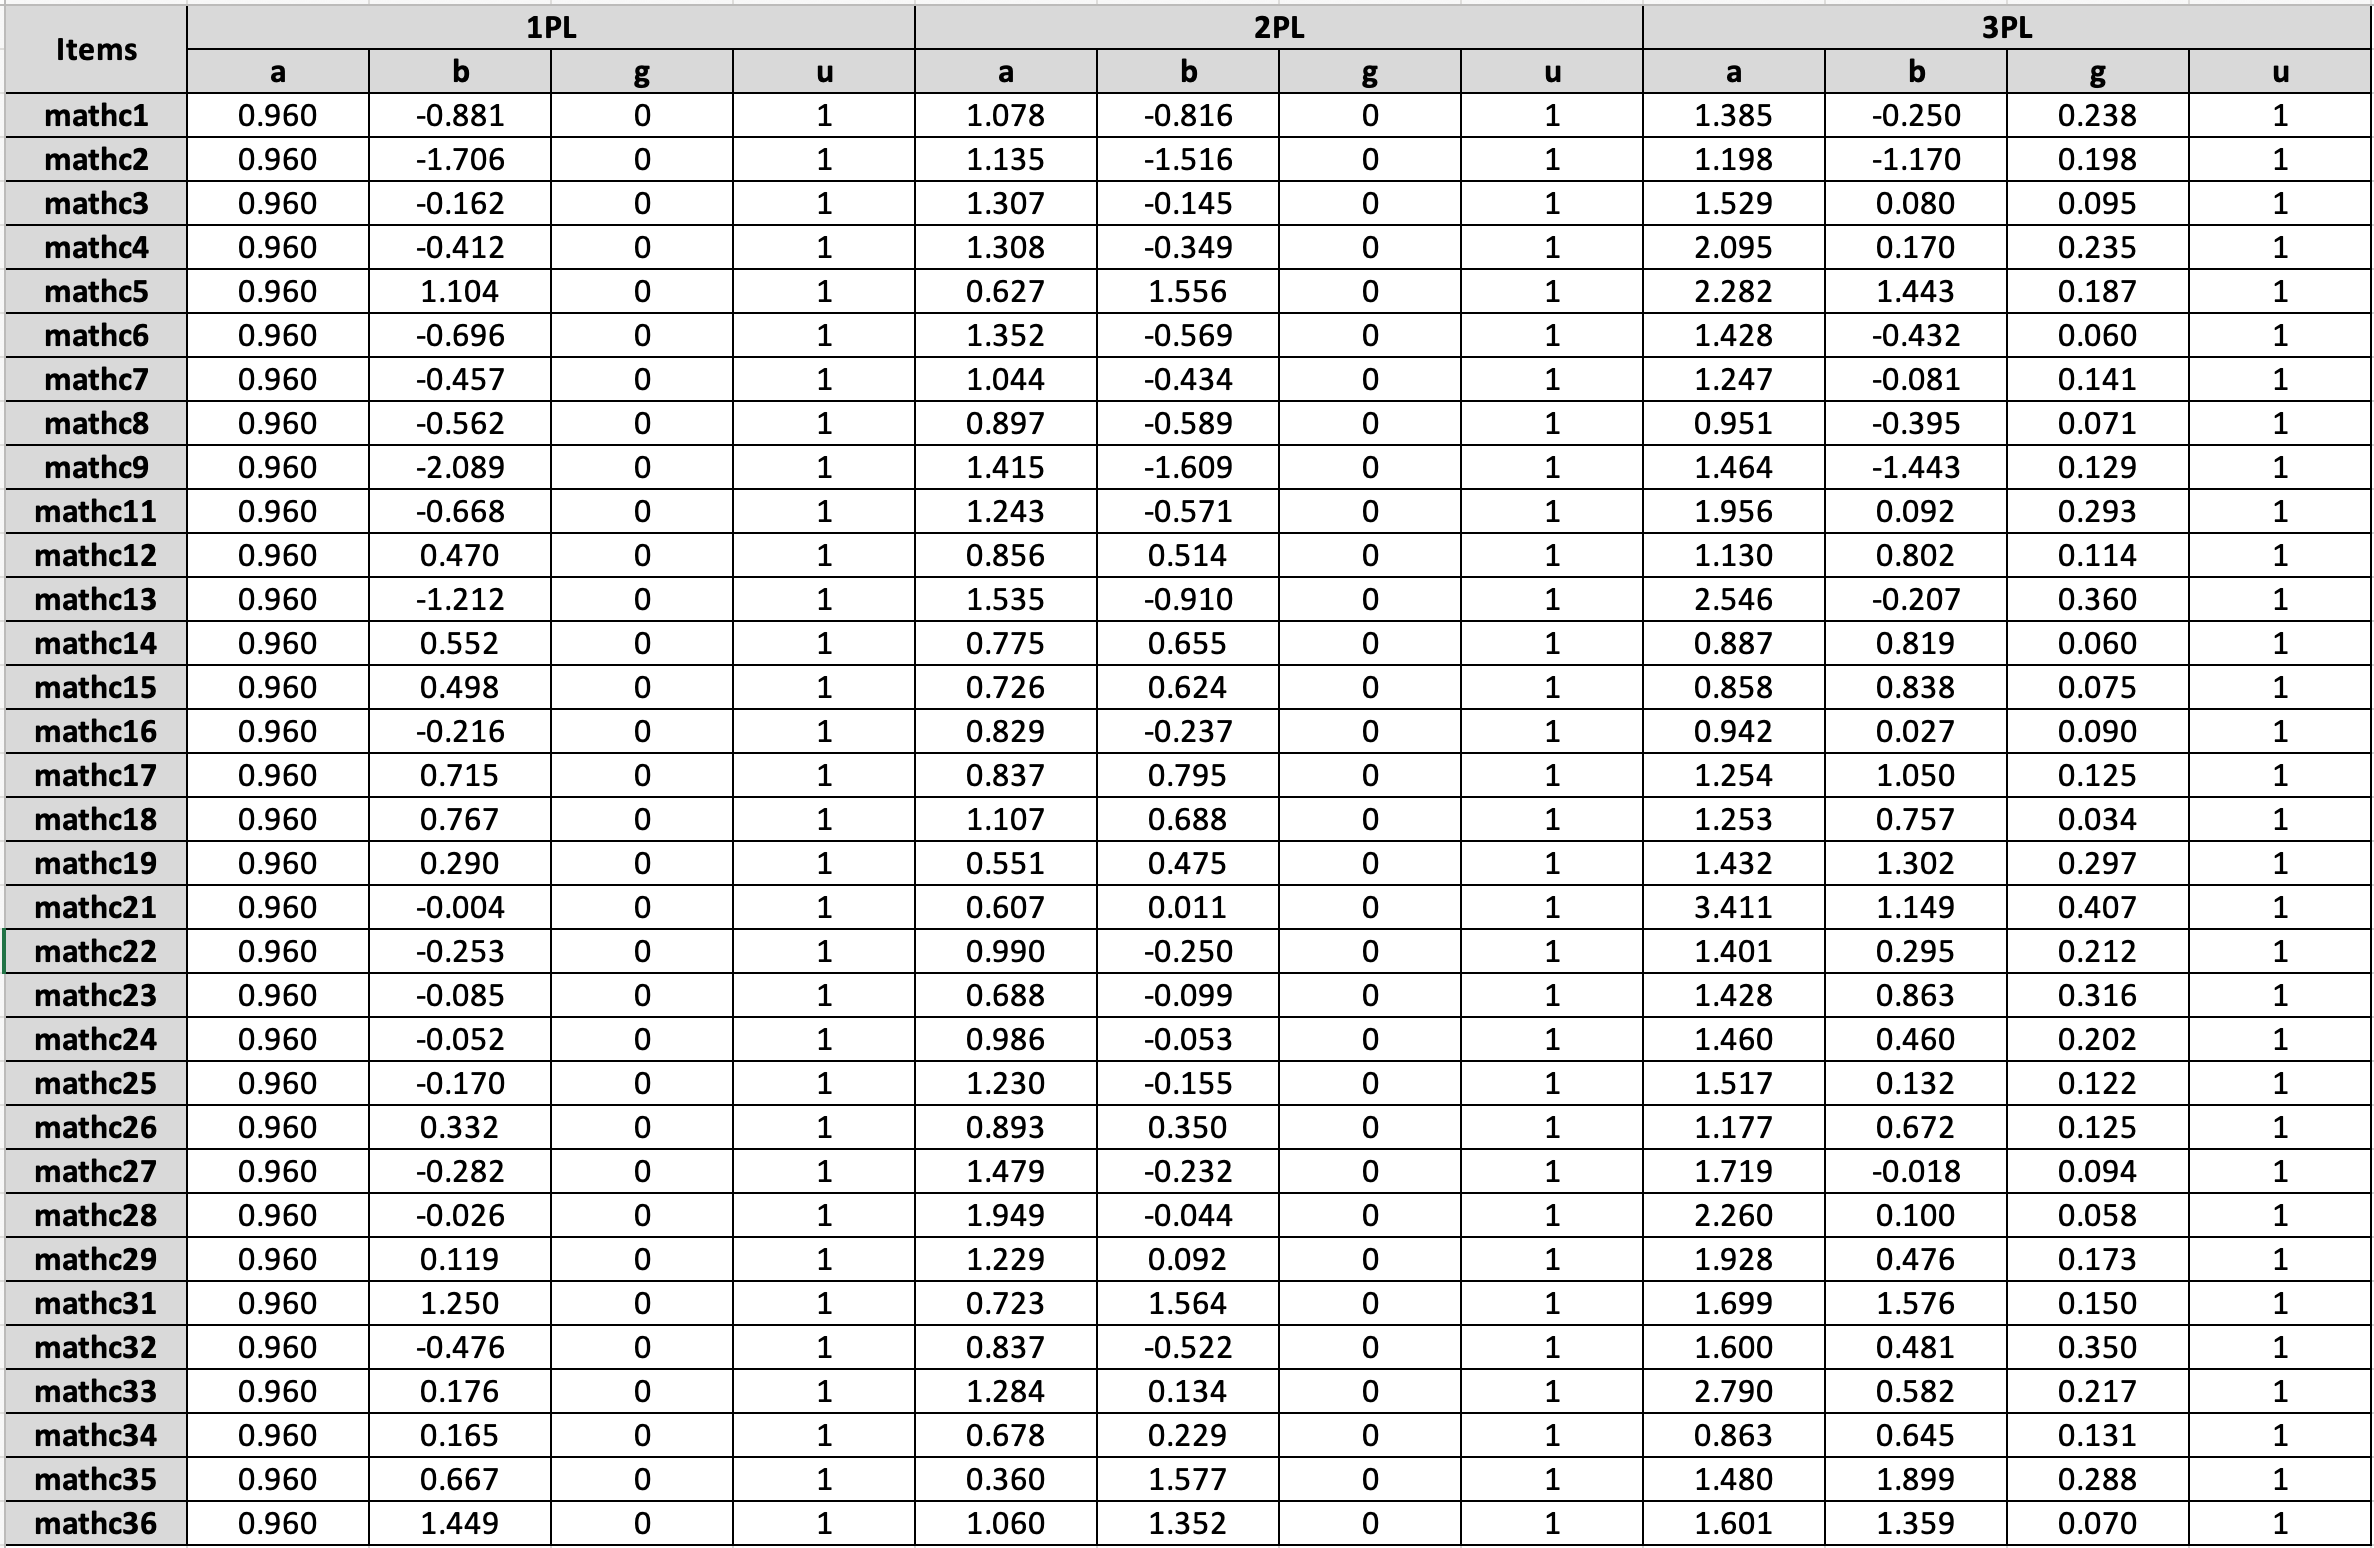
\includegraphics{all_estimated_items.png}

Due to the limitation of \texttt{mirt\ package}, I can't constrain all
the \(\alpha\) to be 1. Rather, I can only set them to be equal across
all the items. Therefore, in the estimation for the 1PL, the estimated
universal \(\alpha\) is .96 here.

\hypertarget{q1-a-1}{%
\subsection{Q1-a-(1)}\label{q1-a-1}}

\emph{Does it appear reasonable to assume all the items having an equal
slope\ldots{}}

\textbf{My Solution:}\\
No.

From a aspect of test development, since this is a test about math
placement, we should expect that items can discriminate students with
different traits well. In addition, comparing the estimated parameters
from \texttt{2PL} model versus \texttt{1PL}, these items' levels of
discrimination spread along a wide range. It is reasonable to have items
with higher levels of discrimination than others.

From a mathematics perspective, since the 1PL model is nested in the 2PL
model, I conducted the \texttt{Likelihood\ Ratio\ Test} to compare the
two models as followed: \[D = -2[ln(L_{1pl})-ln(L_{2pl})] .\]\\
Plug the log likelihood estimated from the above code chunck, then one
can have \(D = 363.2\) at the degree of freedom of
\(df = df_{2pl}-df_{1pl} = 66-34 =32\). Based on the Chi-squared
distribution, the p value is lower than .001. Therefore, 2PL is better
than 1PL, which means the discrimination is preferred.

\hypertarget{q1-a-2}{%
\subsection{Q1-a-(2)}\label{q1-a-2}}

\emph{Does it appear useful to include a guessing parameter in the
model\ldots{}}

\textbf{My Solution:}

Yes, it is useful.

Intuitively, it is reasonable to include a guessing parameter since this
a test with multiple choice and guessing is very possible. In addition,
by looking through all the guessing parameters, one can find that the
\texttt{matchc13}, \texttt{matchc21}, and \texttt{matchc32} do have
quite high guessing rate, i.e., all above .30.

However, in terms of model comparison, when using the LRT test again to
compare the 2PL vs 3PL model, one can have \(D = 28.28\) at \(33\)
degree of freedom, \(P = .701\). Based on the parsimony rule, one should
endorse the simpler model, i.e., the 2PL.

Therefore, my overall conclusion is including a guessing parameter is
useful in this scenario. A practitioner should choose the either model
based on their purpose since these two models do not differ a lot.

\hypertarget{q1-a-3}{%
\subsection{Q1-a-(3)}\label{q1-a-3}}

\emph{Evaluate the goodness of fit of the items with the option of the
chi-square test\ldots{}}

\textbf{My Solution:}

I conduct the item fit analysis on each model and summarize the results
into one table to make the layout concise.

\begin{Shaded}
\begin{Highlighting}[]
\SpecialCharTok{\textgreater{}} \CommentTok{\# get the item fit indices for each model}
\ErrorTok{\textgreater{}}\NormalTok{ item\_fit\_1pl }\OtherTok{\textless{}{-}} \FunctionTok{itemfit}\NormalTok{(irt\_1pl, }\AttributeTok{na.rm =}\NormalTok{ T)}
\SpecialCharTok{\textgreater{}}\NormalTok{ item\_fit\_2pl }\OtherTok{\textless{}{-}} \FunctionTok{itemfit}\NormalTok{(irt\_2pl, }\AttributeTok{na.rm =}\NormalTok{ T)}
\SpecialCharTok{\textgreater{}}\NormalTok{ item\_fit\_3pl }\OtherTok{\textless{}{-}} \FunctionTok{itemfit}\NormalTok{(irt\_3pl, }\AttributeTok{na.rm =}\NormalTok{ T)}
\SpecialCharTok{\textgreater{}} 
\ErrorTok{\textgreater{}} \CommentTok{\# combine all the outputs into one table}
\ErrorTok{\textgreater{}}\NormalTok{ item\_fit\_all }\OtherTok{\textless{}{-}} \FunctionTok{cbind}\NormalTok{(item\_fit\_1pl[,}\FunctionTok{c}\NormalTok{(}\StringTok{"item"}\NormalTok{)],}
\SpecialCharTok{+}                       \FunctionTok{round}\NormalTok{(item\_fit\_1pl[,}\FunctionTok{c}\NormalTok{(}\StringTok{"S\_X2"}\NormalTok{, }\StringTok{"p.S\_X2"}\NormalTok{)],}\DecValTok{4}\NormalTok{),}
\SpecialCharTok{+}                       \FunctionTok{round}\NormalTok{(item\_fit\_2pl[,}\FunctionTok{c}\NormalTok{(}\StringTok{"S\_X2"}\NormalTok{, }\StringTok{"p.S\_X2"}\NormalTok{)],}\DecValTok{4}\NormalTok{),}
\SpecialCharTok{+}                       \FunctionTok{round}\NormalTok{(item\_fit\_3pl[,}\FunctionTok{c}\NormalTok{(}\StringTok{"S\_X2"}\NormalTok{, }\StringTok{"p.S\_X2"}\NormalTok{)],}\DecValTok{4}\NormalTok{))}
\SpecialCharTok{\textgreater{}} \FunctionTok{names}\NormalTok{(item\_fit\_all)[}\DecValTok{1}\NormalTok{] }\OtherTok{\textless{}{-}} \StringTok{"item"}
\SpecialCharTok{\textgreater{}} 
\ErrorTok{\textgreater{}} \CommentTok{\# get all the item fit indices for 1PL, 2PL, and 3PL model}
\ErrorTok{\textgreater{}}\NormalTok{ item\_fit\_all}
\NormalTok{      item     S\_X2 p.S\_X2    S\_X2 p.S\_X2    S\_X2 p.S\_X2}
\DecValTok{1}\NormalTok{   mathc1  }\FloatTok{24.8711} \FloatTok{0.4128} \FloatTok{23.0566} \FloatTok{0.4575} \FloatTok{23.8800} \FloatTok{0.3536}
\DecValTok{2}\NormalTok{   mathc2  }\FloatTok{28.1234} \FloatTok{0.2112} \FloatTok{30.4743} \FloatTok{0.1074} \FloatTok{28.6024} \FloatTok{0.1239}
\DecValTok{3}\NormalTok{   mathc3  }\FloatTok{27.2722} \FloatTok{0.2919} \FloatTok{22.4566} \FloatTok{0.4929} \FloatTok{21.7064} \FloatTok{0.4775}
\DecValTok{4}\NormalTok{   mathc4  }\FloatTok{26.5449} \FloatTok{0.3261} \FloatTok{19.2254} \FloatTok{0.6314} \FloatTok{17.4558} \FloatTok{0.6831}
\DecValTok{5}\NormalTok{   mathc5  }\FloatTok{97.3404} \FloatTok{0.0000} \FloatTok{52.8362} \FloatTok{0.0014} \FloatTok{39.3238} \FloatTok{0.0183}
\DecValTok{6}\NormalTok{   mathc6  }\FloatTok{35.2844} \FloatTok{0.0643} \FloatTok{26.8461} \FloatTok{0.2171} \FloatTok{23.9949} \FloatTok{0.2933}
\DecValTok{7}\NormalTok{   mathc7  }\FloatTok{30.6375} \FloatTok{0.1645} \FloatTok{30.4324} \FloatTok{0.1708} \FloatTok{30.8269} \FloatTok{0.1271}
\DecValTok{8}\NormalTok{   mathc8  }\FloatTok{31.1674} \FloatTok{0.1490} \FloatTok{31.5235} \FloatTok{0.1393} \FloatTok{23.0747} \FloatTok{0.4564}
\DecValTok{9}\NormalTok{   mathc9  }\FloatTok{31.5513} \FloatTok{0.0854} \FloatTok{16.4299} \FloatTok{0.6896} \FloatTok{12.8670} \FloatTok{0.7994}
\DecValTok{10}\NormalTok{ mathc11  }\FloatTok{24.7300} \FloatTok{0.4205} \FloatTok{17.4787} \FloatTok{0.7364} \FloatTok{16.8747} \FloatTok{0.7187}
\DecValTok{11}\NormalTok{ mathc12  }\FloatTok{23.5755} \FloatTok{0.4861} \FloatTok{22.8300} \FloatTok{0.5298} \FloatTok{20.6982} \FloatTok{0.5995}
\DecValTok{12}\NormalTok{ mathc13  }\FloatTok{35.9083} \FloatTok{0.0422} \FloatTok{24.6484} \FloatTok{0.2627} \FloatTok{19.3900} \FloatTok{0.3682}
\DecValTok{13}\NormalTok{ mathc14  }\FloatTok{27.5382} \FloatTok{0.2800} \FloatTok{23.1188} \FloatTok{0.5128} \FloatTok{20.5069} \FloatTok{0.6112}
\DecValTok{14}\NormalTok{ mathc15  }\FloatTok{33.5261} \FloatTok{0.0934} \FloatTok{21.0409} \FloatTok{0.6903} \FloatTok{17.2351} \FloatTok{0.7976}
\DecValTok{15}\NormalTok{ mathc16  }\FloatTok{26.6813} \FloatTok{0.3195} \FloatTok{25.3271} \FloatTok{0.3882} \FloatTok{22.7550} \FloatTok{0.5343}
\DecValTok{16}\NormalTok{ mathc17  }\FloatTok{21.2673} \FloatTok{0.6229} \FloatTok{17.9679} \FloatTok{0.8046} \FloatTok{17.1584} \FloatTok{0.8014}
\DecValTok{17}\NormalTok{ mathc18  }\FloatTok{21.5747} \FloatTok{0.6046} \FloatTok{22.3173} \FloatTok{0.5012} \FloatTok{19.1247} \FloatTok{0.6376}
\DecValTok{18}\NormalTok{ mathc19  }\FloatTok{54.0475} \FloatTok{0.0004} \FloatTok{20.7629} \FloatTok{0.7058} \FloatTok{20.1995} \FloatTok{0.6854}
\DecValTok{19}\NormalTok{ mathc21  }\FloatTok{61.7627} \FloatTok{0.0000} \FloatTok{33.2577} \FloatTok{0.1247} \FloatTok{23.3450} \FloatTok{0.4408}
\DecValTok{20}\NormalTok{ mathc22  }\FloatTok{20.4045} \FloatTok{0.6736} \FloatTok{20.4046} \FloatTok{0.6736} \FloatTok{20.8114} \FloatTok{0.5926}
\DecValTok{21}\NormalTok{ mathc23  }\FloatTok{20.8365} \FloatTok{0.6483} \FloatTok{14.4939} \FloatTok{0.9524} \FloatTok{13.5269} \FloatTok{0.9566}
\DecValTok{22}\NormalTok{ mathc24  }\FloatTok{20.9306} \FloatTok{0.6428} \FloatTok{21.0813} \FloatTok{0.6339} \FloatTok{21.0628} \FloatTok{0.5773}
\DecValTok{23}\NormalTok{ mathc25  }\FloatTok{24.9448} \FloatTok{0.4088} \FloatTok{21.3330} \FloatTok{0.5608} \FloatTok{21.4360} \FloatTok{0.4939}
\DecValTok{24}\NormalTok{ mathc26  }\FloatTok{19.3543} \FloatTok{0.7328} \FloatTok{17.6730} \FloatTok{0.8186} \FloatTok{18.2240} \FloatTok{0.7452}
\DecValTok{25}\NormalTok{ mathc27  }\FloatTok{45.0529} \FloatTok{0.0057} \FloatTok{29.1187} \FloatTok{0.1112} \FloatTok{27.4429} \FloatTok{0.1567}
\DecValTok{26}\NormalTok{ mathc28  }\FloatTok{65.4501} \FloatTok{0.0000} \FloatTok{24.1670} \FloatTok{0.2352} \FloatTok{23.9470} \FloatTok{0.1982}
\DecValTok{27}\NormalTok{ mathc29  }\FloatTok{20.6986} \FloatTok{0.6564} \FloatTok{16.3725} \FloatTok{0.8389} \FloatTok{14.2529} \FloatTok{0.8923}
\DecValTok{28}\NormalTok{ mathc31  }\FloatTok{38.2013} \FloatTok{0.0242} \FloatTok{24.7382} \FloatTok{0.4771} \FloatTok{22.2939} \FloatTok{0.5026}
\DecValTok{29}\NormalTok{ mathc32  }\FloatTok{26.7508} \FloatTok{0.3162} \FloatTok{22.5725} \FloatTok{0.5451} \FloatTok{21.6350} \FloatTok{0.5424}
\DecValTok{30}\NormalTok{ mathc33  }\FloatTok{29.0666} \FloatTok{0.2176} \FloatTok{21.2045} \FloatTok{0.5686}  \FloatTok{8.0644} \FloatTok{0.9949}
\DecValTok{31}\NormalTok{ mathc34  }\FloatTok{37.3521} \FloatTok{0.0403} \FloatTok{26.8718} \FloatTok{0.3623} \FloatTok{24.8798} \FloatTok{0.4123}
\DecValTok{32}\NormalTok{ mathc35 }\FloatTok{109.6358} \FloatTok{0.0000} \FloatTok{32.7703} \FloatTok{0.2048} \FloatTok{35.3966} \FloatTok{0.1033}
\DecValTok{33}\NormalTok{ mathc36  }\FloatTok{28.9987} \FloatTok{0.2202} \FloatTok{25.1823} \FloatTok{0.3410} \FloatTok{23.7681} \FloatTok{0.3595}
\end{Highlighting}
\end{Shaded}

Item \texttt{mathc5} shows bad item fit in all three models. In
addition, \texttt{matchc19}, \texttt{matchc21}, \texttt{matchc27},
\texttt{matchc28}, \texttt{matchc31}, \texttt{matchc34}, and
`\texttt{matchc35} show bad fit in 1PL model only.

\hypertarget{q1-a-4}{%
\subsection{Q1-a-(4)}\label{q1-a-4}}

\emph{Evaluate the overall fit of the model. Which model do you prefer
for this data?\ldots{}}

\textbf{My Solution:}

\begin{Shaded}
\begin{Highlighting}[]
\SpecialCharTok{\textgreater{}} \CommentTok{\# get the fit indices for 1PL model}
\ErrorTok{\textgreater{}} \FunctionTok{M2}\NormalTok{(irt\_1pl, }\AttributeTok{na.rm =}\NormalTok{ T)}
\NormalTok{            M2  df p      RMSEA    RMSEA\_5   RMSEA\_95      SRMSR       TLI}
\NormalTok{stats }\FloatTok{992.2492} \DecValTok{527} \DecValTok{0} \FloatTok{0.03104487} \FloatTok{0.02805368} \FloatTok{0.03398001} \FloatTok{0.05781072} \FloatTok{0.9632371}
\NormalTok{            CFI}
\NormalTok{stats }\FloatTok{0.9633067}
\SpecialCharTok{\textgreater{}} 
\ErrorTok{\textgreater{}} \CommentTok{\# get the fit indices for 2PL model}
\ErrorTok{\textgreater{}} \FunctionTok{M2}\NormalTok{(irt\_2pl, }\AttributeTok{na.rm =}\NormalTok{ T)}
\NormalTok{            M2  df            p      RMSEA    RMSEA\_5   RMSEA\_95      SRMSR}
\NormalTok{stats }\FloatTok{678.0246} \DecValTok{495} \FloatTok{7.852727e{-}08} \FloatTok{0.02009113} \FloatTok{0.01617592} \FloatTok{0.02371771} \FloatTok{0.03274386}
\NormalTok{            TLI       CFI}
\NormalTok{stats }\FloatTok{0.9846029} \FloatTok{0.9855652}
\SpecialCharTok{\textgreater{}} 
\ErrorTok{\textgreater{}} \CommentTok{\# get the fit indices for 3PL model}
\ErrorTok{\textgreater{}} \FunctionTok{M2}\NormalTok{(irt\_3pl, }\AttributeTok{na.rm =}\NormalTok{ T)}
\NormalTok{            M2  df            p      RMSEA    RMSEA\_5   RMSEA\_95      SRMSR}
\NormalTok{stats }\FloatTok{604.7095} \DecValTok{462} \FloatTok{8.359281e{-}06} \FloatTok{0.01836359} \FloatTok{0.01400902} \FloatTok{0.02228458} \FloatTok{0.03106851}
\NormalTok{            TLI       CFI}
\NormalTok{stats }\FloatTok{0.9871369} \FloatTok{0.9887448}
\end{Highlighting}
\end{Shaded}

Past studies have recommended that a TLI of or above .95, a CFI of or
above .95, an RMSEA of or below .05, and an SRMR of or below .05 could
indicate a very good fit. Based on those criteria, all three model
demonstrate very good model fit.

Next, by conducting the Likelihood Ratio Test (LRT) on 1PL vs.~2PL and
2PL vs.~3PL (finished in \texttt{Q1-a-(1)} and \texttt{Q1-a-(2)}), 2PL
is preferred since it is significantly different from 1PL. In addition,
LRT shows there is no significant difference in 2PL and 3PL. Based on
the parsimony rule, I prefer 2PL model on this data.

\hypertarget{q1-a-5}{%
\subsection{Q1-a-(5)}\label{q1-a-5}}

\emph{Using the estimates obtained from the model you choose in
part\ldots{}}

\textbf{My Solution:}

In the selected 2PL model, \texttt{matchc\ 28} shows the highest level
of discrimination with \(\alpha = 1.949\), and \texttt{matchc\ 35} has
the lowest level of discrimination.

Next, to find the most informative item on a given trait level, I write
a function that automatically search for the targeted item.

\begin{Shaded}
\begin{Highlighting}[]
\SpecialCharTok{\textgreater{}} \CommentTok{\# write a function to find the most informative item for a given trait}
\ErrorTok{\textgreater{}} 
\ErrorTok{\textgreater{}}\NormalTok{ most\_info }\OtherTok{\textless{}{-}} \ControlFlowTok{function}\NormalTok{(irt\_model, trait)\{}
\SpecialCharTok{+}   \CommentTok{\# irt\_model can be any estimated IRT model}
\SpecialCharTok{+}   \CommentTok{\# trait can be any given trait level}
\SpecialCharTok{+}\NormalTok{   a }\OtherTok{\textless{}{-}} \DecValTok{0}
\SpecialCharTok{+}\NormalTok{   item\_num }\OtherTok{\textless{}{-}} \DecValTok{0}
\SpecialCharTok{+}   \ControlFlowTok{for}\NormalTok{ (i }\ControlFlowTok{in} \DecValTok{1}\SpecialCharTok{:}\DecValTok{33}\NormalTok{)\{}
\SpecialCharTok{+}     \CommentTok{\# extract the item information at a given trait}
\SpecialCharTok{+}\NormalTok{     info\_temp }\OtherTok{\textless{}{-}} \FunctionTok{iteminfo}\NormalTok{(}\FunctionTok{extract.item}\NormalTok{(irt\_model, i), trait)}
\SpecialCharTok{+}     \CommentTok{\# dynamically updated the best target}
\SpecialCharTok{+}     \ControlFlowTok{if}\NormalTok{ (info\_temp }\SpecialCharTok{\textgreater{}}\NormalTok{ a)\{}
\SpecialCharTok{+}\NormalTok{       a }\OtherTok{\textless{}{-}}\NormalTok{ info\_temp}
\SpecialCharTok{+}\NormalTok{       item\_num }\OtherTok{\textless{}{-}}\NormalTok{ i}
\SpecialCharTok{+}\NormalTok{     \}}
\SpecialCharTok{+}\NormalTok{   \}}
\SpecialCharTok{+}\NormalTok{   out }\OtherTok{\textless{}{-}} \FunctionTok{list}\NormalTok{(}\AttributeTok{item\_num =}\NormalTok{ item\_num, }
\SpecialCharTok{+}               \AttributeTok{info\_value =}\NormalTok{ a)}
\SpecialCharTok{+}   \FunctionTok{return}\NormalTok{(out)}
\SpecialCharTok{+}\NormalTok{ \}}
\end{Highlighting}
\end{Shaded}

Then, I applied this function to find the most informative items on the
given trait levels of \(\theta = -1.5\), \(\theta = 0\), and
\(\theta = 1.5\).

\begin{Shaded}
\begin{Highlighting}[]
\SpecialCharTok{\textgreater{}} \CommentTok{\# using a for loop to get all results in one sitting}
\ErrorTok{\textgreater{}} \ControlFlowTok{for}\NormalTok{ (theta }\ControlFlowTok{in} \FunctionTok{c}\NormalTok{(}\SpecialCharTok{{-}}\FloatTok{1.5}\NormalTok{, }\DecValTok{0}\NormalTok{, }\FloatTok{1.5}\NormalTok{))\{}
\SpecialCharTok{+}\NormalTok{   theta\_out }\OtherTok{\textless{}{-}} \FunctionTok{most\_info}\NormalTok{(irt\_2pl, theta)}
\SpecialCharTok{+}   \FunctionTok{print}\NormalTok{(}\FunctionTok{paste0}\NormalTok{(}\StringTok{"The most informative item on given trait theta="}\NormalTok{, theta,}\StringTok{" is the item "}\NormalTok{, theta\_out}\SpecialCharTok{$}\NormalTok{item\_num, }\StringTok{", i.e., the "}\NormalTok{, item\_fit\_2pl}\SpecialCharTok{$}\NormalTok{item[theta\_out}\SpecialCharTok{$}\NormalTok{item\_num]))}
\SpecialCharTok{+}   \FunctionTok{print}\NormalTok{(}\FunctionTok{paste0}\NormalTok{(}\StringTok{"     with the infomation value of "}\NormalTok{, }\FunctionTok{round}\NormalTok{(theta\_out}\SpecialCharTok{$}\NormalTok{info\_value,}\DecValTok{4}\NormalTok{)))}
\SpecialCharTok{+}\NormalTok{ \}}
\NormalTok{[}\DecValTok{1}\NormalTok{] }\StringTok{"The most informative item on given trait theta={-}1.5 is the item 9, i.e., the mathc9"}
\NormalTok{[}\DecValTok{1}\NormalTok{] }\StringTok{"     with the infomation value of 0.4978"}
\NormalTok{[}\DecValTok{1}\NormalTok{] }\StringTok{"The most informative item on given trait theta=0 is the item 26, i.e., the mathc28"}
\NormalTok{[}\DecValTok{1}\NormalTok{] }\StringTok{"     with the infomation value of 0.9477"}
\NormalTok{[}\DecValTok{1}\NormalTok{] }\StringTok{"The most informative item on given trait theta=1.5 is the item 33, i.e., the mathc36"}
\NormalTok{[}\DecValTok{1}\NormalTok{] }\StringTok{"     with the infomation value of 0.2789"}
\end{Highlighting}
\end{Shaded}

As shown above, the most informative item on \(\theta = -1.5\) is the
item \texttt{matchc9}. The most informative item on \(\theta = 0\) is
the item \texttt{matchc28}. The most informative item on
\(\theta = 1.5\) is the item \texttt{matchc36}.

\hypertarget{q1-b}{%
\subsection{Q1-b}\label{q1-b}}

\emph{Using the estimates obtained from the model you choose in
part\ldots{}}

\textbf{My Solution:} As discussed above, I used the 2PL model to
conduct the analysis. First, I got all the expected score (i.e., true
score) for each trait levels using the \texttt{expected.test()}
function. Second, I located the trait score with a corresponding true
score 20.

\begin{Shaded}
\begin{Highlighting}[]
\SpecialCharTok{\textgreater{}} \CommentTok{\# get the thetas from this sample}
\ErrorTok{\textgreater{}}\NormalTok{ theta }\OtherTok{\textless{}{-}} \FunctionTok{fscores}\NormalTok{(irt\_2pl, }\AttributeTok{method =} \StringTok{\textquotesingle{}EAP\textquotesingle{}}\NormalTok{)}
\SpecialCharTok{\textgreater{}} 
\ErrorTok{\textgreater{}} \CommentTok{\# re{-}define a vector of trait levles}
\ErrorTok{\textgreater{}}\NormalTok{ theta\_tempt }\OtherTok{\textless{}{-}} \FunctionTok{as.matrix}\NormalTok{(}\FunctionTok{seq}\NormalTok{(}\SpecialCharTok{{-}}\DecValTok{6}\NormalTok{,}\DecValTok{6}\NormalTok{,}\FloatTok{0.01}\NormalTok{))}
\SpecialCharTok{\textgreater{}} 
\ErrorTok{\textgreater{}} \CommentTok{\# find the trait level who have the true score of 20}
\ErrorTok{\textgreater{}}\NormalTok{ tscore }\OtherTok{\textless{}{-}} \FunctionTok{expected.test}\NormalTok{(irt\_2pl, theta\_tempt)}
\SpecialCharTok{\textgreater{}}\NormalTok{ theta\_20 }\OtherTok{\textless{}{-}} \FunctionTok{mean}\NormalTok{(theta\_tempt[tscore }\SpecialCharTok{\textgreater{}}\FloatTok{19.9} \SpecialCharTok{\&}\NormalTok{ tscore }\SpecialCharTok{\textless{}}\FloatTok{20.1}\NormalTok{])}
\SpecialCharTok{\textgreater{}} 
\ErrorTok{\textgreater{}} \CommentTok{\# plot the TCC curve!}
\ErrorTok{\textgreater{}} \FunctionTok{plot}\NormalTok{(theta\_tempt, tscore, }\AttributeTok{type =} \StringTok{"l"}\NormalTok{, }\AttributeTok{col=}\StringTok{"red"}\NormalTok{,}
\SpecialCharTok{+}      \AttributeTok{xlim =} \FunctionTok{c}\NormalTok{(}\SpecialCharTok{{-}}\DecValTok{6}\NormalTok{,}\DecValTok{6}\NormalTok{),}
\SpecialCharTok{+}      \AttributeTok{main=}\StringTok{"Total Expected Score (i.e., TCC)"}\NormalTok{,}
\SpecialCharTok{+}      \AttributeTok{xlab=}\StringTok{"Theta Levels"}\NormalTok{, }\AttributeTok{ylab=}\StringTok{"True Score"}\NormalTok{)}
\SpecialCharTok{\textgreater{}} \FunctionTok{abline}\NormalTok{(}\AttributeTok{h =} \DecValTok{20}\NormalTok{,}\AttributeTok{col=}\StringTok{"blue"}\NormalTok{,}\AttributeTok{lty=}\DecValTok{2}\NormalTok{)}
\SpecialCharTok{\textgreater{}} \FunctionTok{abline}\NormalTok{(}\AttributeTok{v =} \FloatTok{0.413}\NormalTok{,}\AttributeTok{col=}\StringTok{"blue"}\NormalTok{,}\AttributeTok{lty=}\DecValTok{2}\NormalTok{)}
\SpecialCharTok{\textgreater{}} \FunctionTok{grid}\NormalTok{()}
\end{Highlighting}
\end{Shaded}

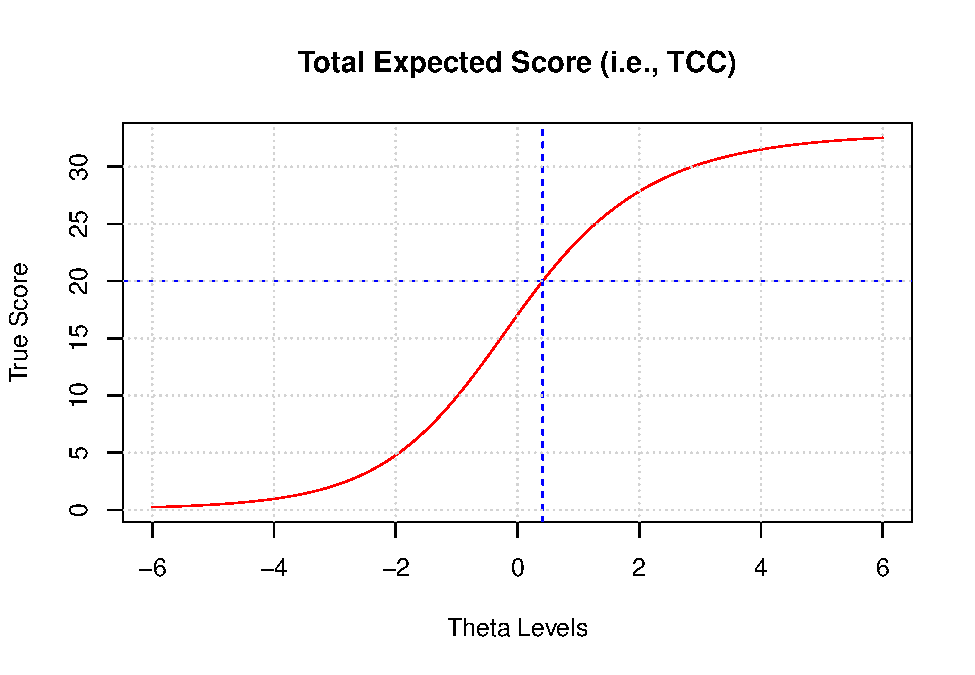
\includegraphics{Assignment_4_files/figure-latex/unnamed-chunk-12-1.pdf}
The TCC curve shows that the trait level of true score 20 is 0.41.
Therefore, we need to select 10 items to have the maximum information on
the 0.41.

Next, I try to get the information values of each item on 0.41 and sort
these values in decreasing order. Finally, select the first ten items to
make the shorter test.

\begin{Shaded}
\begin{Highlighting}[]
\SpecialCharTok{\textgreater{}}\NormalTok{ info\_set }\OtherTok{\textless{}{-}} \FunctionTok{c}\NormalTok{()}
\SpecialCharTok{\textgreater{}} \CommentTok{\# using a for loop to get all info value at this given trait}
\ErrorTok{\textgreater{}} \ControlFlowTok{for}\NormalTok{ (i }\ControlFlowTok{in} \DecValTok{1}\SpecialCharTok{:}\DecValTok{33}\NormalTok{) \{}
\SpecialCharTok{+}\NormalTok{   info\_tempt }\OtherTok{\textless{}{-}} \FunctionTok{iteminfo}\NormalTok{(}\FunctionTok{extract.item}\NormalTok{(irt\_2pl, i), theta\_20)}
\SpecialCharTok{+}\NormalTok{   info\_set[i] }\OtherTok{\textless{}{-}}\NormalTok{ info\_tempt}
\SpecialCharTok{+}\NormalTok{ \}}
\SpecialCharTok{\textgreater{}} \CommentTok{\# make a new df}
\ErrorTok{\textgreater{}}\NormalTok{ info\_matrix }\OtherTok{\textless{}{-}} \FunctionTok{data.frame}\NormalTok{(}
\SpecialCharTok{+}   \AttributeTok{item =}\NormalTok{ item\_fit\_2pl[,}\FunctionTok{c}\NormalTok{(}\StringTok{"item"}\NormalTok{)],}
\SpecialCharTok{+}   \AttributeTok{info\_value =}\NormalTok{ info\_set}
\SpecialCharTok{+}\NormalTok{ )}
\SpecialCharTok{\textgreater{}} \CommentTok{\# sort this df in decreasing order}
\ErrorTok{\textgreater{}}\NormalTok{ info\_matrix }\OtherTok{\textless{}{-}}\NormalTok{ info\_matrix[}\FunctionTok{order}\NormalTok{(}\SpecialCharTok{{-}}\NormalTok{info\_matrix}\SpecialCharTok{$}\NormalTok{info\_value),]}
\SpecialCharTok{\textgreater{}} \CommentTok{\# get the first 10 items}
\ErrorTok{\textgreater{}}\NormalTok{ info\_matrix[}\FunctionTok{c}\NormalTok{(}\DecValTok{1}\SpecialCharTok{:}\DecValTok{10}\NormalTok{),]}
\NormalTok{      item info\_value}
\DecValTok{26}\NormalTok{ mathc28  }\FloatTok{0.7855788}
\DecValTok{25}\NormalTok{ mathc27  }\FloatTok{0.4398556}
\DecValTok{30}\NormalTok{ mathc33  }\FloatTok{0.3991881}
\DecValTok{3}\NormalTok{   mathc3  }\FloatTok{0.3752177}
\DecValTok{27}\NormalTok{ mathc29  }\FloatTok{0.3633219}
\DecValTok{4}\NormalTok{   mathc4  }\FloatTok{0.3375869}
\DecValTok{23}\NormalTok{ mathc25  }\FloatTok{0.3359483}
\DecValTok{6}\NormalTok{   mathc6  }\FloatTok{0.3034735}
\DecValTok{17}\NormalTok{ mathc18  }\FloatTok{0.2993334}
\DecValTok{10}\NormalTok{ mathc11  }\FloatTok{0.2719404}
\end{Highlighting}
\end{Shaded}

As shown above, I will select these ten items to create a shorter
version of test.

\begin{Shaded}
\begin{Highlighting}[]
\SpecialCharTok{\textgreater{}}\NormalTok{ df\_short }\OtherTok{\textless{}{-}}\NormalTok{ df[,}\FunctionTok{which}\NormalTok{(}\FunctionTok{names}\NormalTok{(df) }\SpecialCharTok{\%in\%}\NormalTok{ info\_matrix}\SpecialCharTok{$}\NormalTok{item[}\DecValTok{1}\SpecialCharTok{:}\DecValTok{10}\NormalTok{])]}
\SpecialCharTok{\textgreater{}} \CommentTok{\# fit 2PL on this short test}
\ErrorTok{\textgreater{}}\NormalTok{ irt\_2pl\_short }\OtherTok{\textless{}{-}} \FunctionTok{mirt}\NormalTok{(df\_short, }\AttributeTok{model =} \DecValTok{1}\NormalTok{, }\AttributeTok{itemtype =} \StringTok{"2PL"}\NormalTok{, }\AttributeTok{SE=}\NormalTok{T)}
\NormalTok{Iteration}\SpecialCharTok{:} \DecValTok{1}\NormalTok{, Log}\SpecialCharTok{{-}}\NormalTok{Lik}\SpecialCharTok{:} \SpecialCharTok{{-}}\FloatTok{6358.356}\NormalTok{, Max}\SpecialCharTok{{-}}\NormalTok{Change}\SpecialCharTok{:} \FloatTok{0.54171}\NormalTok{Iteration}\SpecialCharTok{:} \DecValTok{2}\NormalTok{, Log}\SpecialCharTok{{-}}\NormalTok{Lik}\SpecialCharTok{:} \SpecialCharTok{{-}}\FloatTok{6291.212}\NormalTok{, Max}\SpecialCharTok{{-}}\NormalTok{Change}\SpecialCharTok{:} \FloatTok{0.32404}\NormalTok{Iteration}\SpecialCharTok{:} \DecValTok{3}\NormalTok{, Log}\SpecialCharTok{{-}}\NormalTok{Lik}\SpecialCharTok{:} \SpecialCharTok{{-}}\FloatTok{6274.259}\NormalTok{, Max}\SpecialCharTok{{-}}\NormalTok{Change}\SpecialCharTok{:} \FloatTok{0.19571}\NormalTok{Iteration}\SpecialCharTok{:} \DecValTok{4}\NormalTok{, Log}\SpecialCharTok{{-}}\NormalTok{Lik}\SpecialCharTok{:} \SpecialCharTok{{-}}\FloatTok{6269.151}\NormalTok{, Max}\SpecialCharTok{{-}}\NormalTok{Change}\SpecialCharTok{:} \FloatTok{0.11830}\NormalTok{Iteration}\SpecialCharTok{:} \DecValTok{5}\NormalTok{, Log}\SpecialCharTok{{-}}\NormalTok{Lik}\SpecialCharTok{:} \SpecialCharTok{{-}}\FloatTok{6267.498}\NormalTok{, Max}\SpecialCharTok{{-}}\NormalTok{Change}\SpecialCharTok{:} \FloatTok{0.07200}\NormalTok{Iteration}\SpecialCharTok{:} \DecValTok{6}\NormalTok{, Log}\SpecialCharTok{{-}}\NormalTok{Lik}\SpecialCharTok{:} \SpecialCharTok{{-}}\FloatTok{6266.925}\NormalTok{, Max}\SpecialCharTok{{-}}\NormalTok{Change}\SpecialCharTok{:} \FloatTok{0.04343}\NormalTok{Iteration}\SpecialCharTok{:} \DecValTok{7}\NormalTok{, Log}\SpecialCharTok{{-}}\NormalTok{Lik}\SpecialCharTok{:} \SpecialCharTok{{-}}\FloatTok{6266.665}\NormalTok{, Max}\SpecialCharTok{{-}}\NormalTok{Change}\SpecialCharTok{:} \FloatTok{0.01914}\NormalTok{Iteration}\SpecialCharTok{:} \DecValTok{8}\NormalTok{, Log}\SpecialCharTok{{-}}\NormalTok{Lik}\SpecialCharTok{:} \SpecialCharTok{{-}}\FloatTok{6266.623}\NormalTok{, Max}\SpecialCharTok{{-}}\NormalTok{Change}\SpecialCharTok{:} \FloatTok{0.01179}\NormalTok{Iteration}\SpecialCharTok{:} \DecValTok{9}\NormalTok{, Log}\SpecialCharTok{{-}}\NormalTok{Lik}\SpecialCharTok{:} \SpecialCharTok{{-}}\FloatTok{6266.606}\NormalTok{, Max}\SpecialCharTok{{-}}\NormalTok{Change}\SpecialCharTok{:} \FloatTok{0.00719}\NormalTok{Iteration}\SpecialCharTok{:} \DecValTok{10}\NormalTok{, Log}\SpecialCharTok{{-}}\NormalTok{Lik}\SpecialCharTok{:} \SpecialCharTok{{-}}\FloatTok{6266.595}\NormalTok{, Max}\SpecialCharTok{{-}}\NormalTok{Change}\SpecialCharTok{:} \FloatTok{0.00273}\NormalTok{Iteration}\SpecialCharTok{:} \DecValTok{11}\NormalTok{, Log}\SpecialCharTok{{-}}\NormalTok{Lik}\SpecialCharTok{:} \SpecialCharTok{{-}}\FloatTok{6266.593}\NormalTok{, Max}\SpecialCharTok{{-}}\NormalTok{Change}\SpecialCharTok{:} \FloatTok{0.00157}\NormalTok{Iteration}\SpecialCharTok{:} \DecValTok{12}\NormalTok{, Log}\SpecialCharTok{{-}}\NormalTok{Lik}\SpecialCharTok{:} \SpecialCharTok{{-}}\FloatTok{6266.592}\NormalTok{, Max}\SpecialCharTok{{-}}\NormalTok{Change}\SpecialCharTok{:} \FloatTok{0.00106}\NormalTok{Iteration}\SpecialCharTok{:} \DecValTok{13}\NormalTok{, Log}\SpecialCharTok{{-}}\NormalTok{Lik}\SpecialCharTok{:} \SpecialCharTok{{-}}\FloatTok{6266.592}\NormalTok{, Max}\SpecialCharTok{{-}}\NormalTok{Change}\SpecialCharTok{:} \FloatTok{0.00069}\NormalTok{Iteration}\SpecialCharTok{:} \DecValTok{14}\NormalTok{, Log}\SpecialCharTok{{-}}\NormalTok{Lik}\SpecialCharTok{:} \SpecialCharTok{{-}}\FloatTok{6266.592}\NormalTok{, Max}\SpecialCharTok{{-}}\NormalTok{Change}\SpecialCharTok{:} \FloatTok{0.00074}\NormalTok{Iteration}\SpecialCharTok{:} \DecValTok{15}\NormalTok{, Log}\SpecialCharTok{{-}}\NormalTok{Lik}\SpecialCharTok{:} \SpecialCharTok{{-}}\FloatTok{6266.592}\NormalTok{, Max}\SpecialCharTok{{-}}\NormalTok{Change}\SpecialCharTok{:} \FloatTok{0.00066}\NormalTok{Iteration}\SpecialCharTok{:} \DecValTok{16}\NormalTok{, Log}\SpecialCharTok{{-}}\NormalTok{Lik}\SpecialCharTok{:} \SpecialCharTok{{-}}\FloatTok{6266.592}\NormalTok{, Max}\SpecialCharTok{{-}}\NormalTok{Change}\SpecialCharTok{:} \FloatTok{0.00037}\NormalTok{Iteration}\SpecialCharTok{:} \DecValTok{17}\NormalTok{, Log}\SpecialCharTok{{-}}\NormalTok{Lik}\SpecialCharTok{:} \SpecialCharTok{{-}}\FloatTok{6266.591}\NormalTok{, Max}\SpecialCharTok{{-}}\NormalTok{Change}\SpecialCharTok{:} \FloatTok{0.00025}\NormalTok{Iteration}\SpecialCharTok{:} \DecValTok{18}\NormalTok{, Log}\SpecialCharTok{{-}}\NormalTok{Lik}\SpecialCharTok{:} \SpecialCharTok{{-}}\FloatTok{6266.591}\NormalTok{, Max}\SpecialCharTok{{-}}\NormalTok{Change}\SpecialCharTok{:} \FloatTok{0.00016}\NormalTok{Iteration}\SpecialCharTok{:} \DecValTok{19}\NormalTok{, Log}\SpecialCharTok{{-}}\NormalTok{Lik}\SpecialCharTok{:} \SpecialCharTok{{-}}\FloatTok{6266.591}\NormalTok{, Max}\SpecialCharTok{{-}}\NormalTok{Change}\SpecialCharTok{:} \FloatTok{0.00006}

\NormalTok{Calculating information matrix...}
\SpecialCharTok{\textgreater{}}\NormalTok{ irt\_2pl\_short}

\NormalTok{Call}\SpecialCharTok{:}
\FunctionTok{mirt}\NormalTok{(}\AttributeTok{data =}\NormalTok{ df\_short, }\AttributeTok{model =} \DecValTok{1}\NormalTok{, }\AttributeTok{itemtype =} \StringTok{"2PL"}\NormalTok{, }\AttributeTok{SE =}\NormalTok{ T)}

\NormalTok{Full}\SpecialCharTok{{-}}\NormalTok{information item factor analysis with }\DecValTok{1} \FunctionTok{factor}\NormalTok{(s).}
\NormalTok{Converged within }\FloatTok{1e{-}04}\NormalTok{ tolerance after }\DecValTok{19}\NormalTok{ EM iterations.}
\NormalTok{mirt version}\SpecialCharTok{:} \FloatTok{1.40} 
\NormalTok{M}\SpecialCharTok{{-}}\NormalTok{step optimizer}\SpecialCharTok{:}\NormalTok{ BFGS }
\NormalTok{EM acceleration}\SpecialCharTok{:}\NormalTok{ Ramsay }
\NormalTok{Number of rectangular quadrature}\SpecialCharTok{:} \DecValTok{61}
\NormalTok{Latent density type}\SpecialCharTok{:}\NormalTok{ Gaussian }

\NormalTok{Information matrix estimated with method}\SpecialCharTok{:}\NormalTok{ Oakes}
\NormalTok{Second}\SpecialCharTok{{-}}\NormalTok{order test}\SpecialCharTok{:}\NormalTok{ model is a possible local maximum}
\NormalTok{Condition number of information matrix }\OtherTok{=}  \FloatTok{9.291311}

\NormalTok{Log}\SpecialCharTok{{-}}\NormalTok{likelihood }\OtherTok{=} \SpecialCharTok{{-}}\FloatTok{6266.591}
\NormalTok{Estimated parameters}\SpecialCharTok{:} \DecValTok{20} 
\NormalTok{AIC }\OtherTok{=} \FloatTok{12573.18}
\NormalTok{BIC }\OtherTok{=} \FloatTok{12672.18}\NormalTok{; SABIC }\OtherTok{=} \FloatTok{12608.66}
\end{Highlighting}
\end{Shaded}

Now to get the person trait estimation.

\begin{Shaded}
\begin{Highlighting}[]
\SpecialCharTok{\textgreater{}} 
\ErrorTok{\textgreater{}} \FunctionTok{library}\NormalTok{(latticeExtra)}
\SpecialCharTok{\textgreater{}}\NormalTok{ key }\OtherTok{=} \FunctionTok{list}\NormalTok{(}\AttributeTok{colums=}\DecValTok{1}\NormalTok{,}
\SpecialCharTok{+}            \AttributeTok{text=}\FunctionTok{list}\NormalTok{(}\AttributeTok{lab =} \FunctionTok{c}\NormalTok{(}\StringTok{"Original\_20"}\NormalTok{,}\StringTok{"Shorter\_10"}\NormalTok{)),}
\SpecialCharTok{+}            \AttributeTok{lines=}\FunctionTok{list}\NormalTok{(}\AttributeTok{lwd=}\DecValTok{4}\NormalTok{, }\AttributeTok{col=}\FunctionTok{c}\NormalTok{(}\StringTok{"blue"}\NormalTok{,}\StringTok{"lightblue"}\NormalTok{)))}
\SpecialCharTok{\textgreater{}}\NormalTok{ p1 }\OtherTok{\textless{}{-}} \FunctionTok{plot}\NormalTok{(irt\_2pl, }\AttributeTok{type=} \StringTok{"info"}\NormalTok{,}\AttributeTok{key=}\NormalTok{key)}
\SpecialCharTok{\textgreater{}}\NormalTok{ p2 }\OtherTok{\textless{}{-}} \FunctionTok{update}\NormalTok{(}\FunctionTok{plot}\NormalTok{(irt\_2pl\_short, }\AttributeTok{type=}\StringTok{"info"}\NormalTok{), }\AttributeTok{col=}\StringTok{"lightblue"}\NormalTok{)}
\SpecialCharTok{\textgreater{}}\NormalTok{ p1}\SpecialCharTok{+}\NormalTok{p2}
\end{Highlighting}
\end{Shaded}

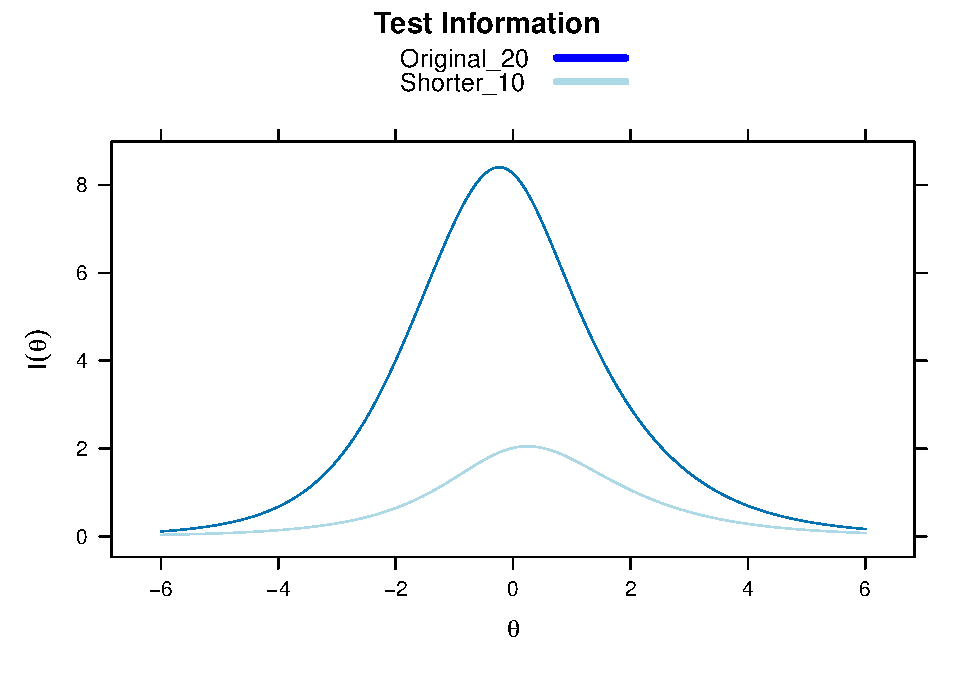
\includegraphics{Assignment_4_files/figure-latex/unnamed-chunk-15-1.pdf}
The plot shows that the peak of shorter test's information is closer to
the target trait level 0.41. However, it provides less information
comparing to the original 20 items test, which means shorter test is
less accurate on estimating the given trait level comparing the to the
original 20 items.

\hypertarget{q1-c}{%
\subsection{Q1-c}\label{q1-c}}

\emph{Assume a student with a true score of 8 on the \ldots{}}

\textbf{My Solution:}

\begin{Shaded}
\begin{Highlighting}[]
\SpecialCharTok{\textgreater{}} \CommentTok{\# get the corresponding true score along the trait scores}
\ErrorTok{\textgreater{}}\NormalTok{ tscore }\OtherTok{\textless{}{-}} \FunctionTok{expected.test}\NormalTok{(irt\_2pl\_short, theta\_tempt)}
\SpecialCharTok{\textgreater{}}\NormalTok{ theta\_8 }\OtherTok{\textless{}{-}} \FunctionTok{mean}\NormalTok{(theta\_tempt[tscore }\SpecialCharTok{\textgreater{}}\FloatTok{7.9} \SpecialCharTok{\&}\NormalTok{ tscore }\SpecialCharTok{\textless{}}\FloatTok{8.1}\NormalTok{])}
\SpecialCharTok{\textgreater{}} \CommentTok{\# plot the TCC }
\ErrorTok{\textgreater{}} \CommentTok{\# plot the TCC curve!}
\ErrorTok{\textgreater{}} \FunctionTok{plot}\NormalTok{(theta\_tempt, tscore, }\AttributeTok{type =} \StringTok{"l"}\NormalTok{, }\AttributeTok{col=}\StringTok{"red"}\NormalTok{,}
\SpecialCharTok{+}      \AttributeTok{xlim =} \FunctionTok{c}\NormalTok{(}\SpecialCharTok{{-}}\DecValTok{6}\NormalTok{,}\DecValTok{6}\NormalTok{),}
\SpecialCharTok{+}      \AttributeTok{main=}\StringTok{"Total Expected Score (i.e., TCC) for Short Test"}\NormalTok{,}
\SpecialCharTok{+}      \AttributeTok{xlab=}\StringTok{"Theta Levels"}\NormalTok{, }\AttributeTok{ylab=}\StringTok{"True Score"}\NormalTok{)}
\SpecialCharTok{\textgreater{}} \FunctionTok{abline}\NormalTok{(}\AttributeTok{h =} \DecValTok{8}\NormalTok{,}\AttributeTok{col=}\StringTok{"blue"}\NormalTok{,}\AttributeTok{lty=}\DecValTok{2}\NormalTok{)}
\SpecialCharTok{\textgreater{}} \FunctionTok{abline}\NormalTok{(}\AttributeTok{v =}\NormalTok{ theta\_8,}\AttributeTok{col=}\StringTok{"blue"}\NormalTok{,}\AttributeTok{lty=}\DecValTok{2}\NormalTok{)}
\SpecialCharTok{\textgreater{}} \FunctionTok{grid}\NormalTok{()}
\end{Highlighting}
\end{Shaded}

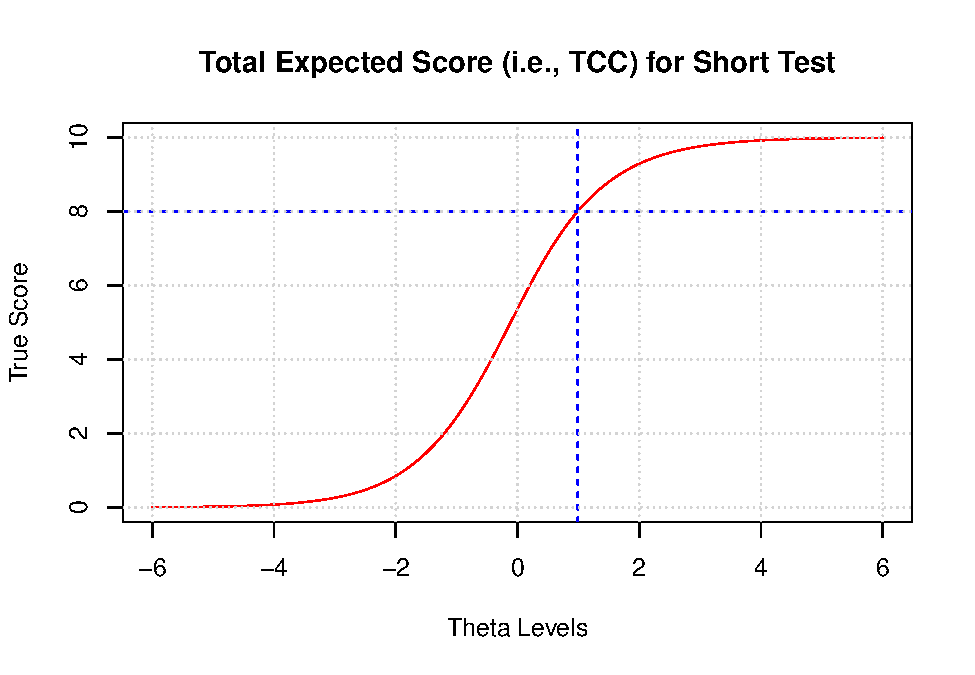
\includegraphics{Assignment_4_files/figure-latex/unnamed-chunk-16-1.pdf}
The plot shows that the corresponding trait level is around 0.99. Next,
I extract the information at this level and calculate the standard
error.

\begin{Shaded}
\begin{Highlighting}[]
\SpecialCharTok{\textgreater{}} \CommentTok{\# get the test info at the theta = 2.255}
\ErrorTok{\textgreater{}}\NormalTok{ test\_info }\OtherTok{\textless{}{-}} \FunctionTok{testinfo}\NormalTok{(irt\_2pl\_short, theta\_tempt)}
\SpecialCharTok{\textgreater{}}\NormalTok{ info\_8 }\OtherTok{\textless{}{-}}\NormalTok{ test\_info[theta\_tempt }\SpecialCharTok{==} \FunctionTok{round}\NormalTok{(theta\_8,}\DecValTok{2}\NormalTok{)]}
\SpecialCharTok{\textgreater{}} 
\ErrorTok{\textgreater{}} \CommentTok{\# calculate the SE based on the relation between the Info and SE}
\ErrorTok{\textgreater{}}\NormalTok{ se\_8 }\OtherTok{\textless{}{-}} \DecValTok{1}\SpecialCharTok{/} \FunctionTok{sqrt}\NormalTok{(info\_8)}
\SpecialCharTok{\textgreater{}}\NormalTok{ se\_8}
\FunctionTok{numeric}\NormalTok{(}\DecValTok{0}\NormalTok{)}
\end{Highlighting}
\end{Shaded}

Based on the all the calculation above, for a student with true score of
8, his/ her corresponding trait level for this short test is 0.99 with
standard error .

\hypertarget{q2}{%
\subsection{Q2}\label{q2}}

\emph{Suppose for three items \ldots{}}

\textbf{My Solution:}\\
From the lecture note, we know that
\[P(\mu_{ij}|S_j)=\frac{\prod_{i=1}^{n}{\epsilon^{\mu_{ij}}}_i}{\sum_{(\mu_{ij})}^{r}{\prod_{i=1}^{n}{\epsilon^{\mu_{ij}}}_i}},\]
where \((\mu_{ij})\) is all the possible response vectors given the
total score is \(r\). The possible response vectors are
\[X_1=[1,1,0], X_2=[1,0,1], X_3=[0,1,1].\]

In Rasch model, since
\[\beta = log(\delta) =log(\frac{1}{\epsilon})=-log(\epsilon), \] one
can have \[\epsilon=e^{(-\beta)}.\] Therefore, we can easily have
\(\epsilon_1 = 4.482\), \(\epsilon_2 = .607\), and
\(\epsilon_3 = .135\).

Based on all the information above, one can have
\[P(X_1|\eta_j)=\frac{\epsilon_1\epsilon_2}{\epsilon_1\epsilon_2+\epsilon_1\epsilon_3+\epsilon_2\epsilon_3}=.798,\]
\[P(X_2|\eta_j)=\frac{\epsilon_1\epsilon_3}{\epsilon_1\epsilon_2+\epsilon_1\epsilon_3+\epsilon_2\epsilon_3}=.178,\]
\[
P(X_3|\eta_j)=\frac{\epsilon_2\epsilon_3}{\epsilon_1\epsilon_2+\epsilon_1\epsilon_3+\epsilon_2\epsilon_3}=.024.\]

\end{document}
